\documentclass[
    a5paper,
    pagesize,
    11pt,
    bibtotoc,
    normalheadings,
    twoside,
    openany,
    chapterprefix,
    DIV=9
]{scrbook}

\usepackage[utf8]{inputenc}
\usepackage{tocloft}
\usepackage{mathtools}
\usepackage{amsfonts}
\usepackage{enumitem}
\usepackage{amsmath}
\usepackage{amsthm}
\usepackage{amssymb}
\usepackage[hmargin=2cm, vmargin=2.5cm]{geometry}
\usepackage{graphicx}
\usepackage{wrapfig}
\usepackage{parskip}
\usepackage{framed}
\usepackage{fancyhdr}
\usepackage{emptypage}
\usepackage{multicol}
\usepackage{imakeidx}
\usepackage[breaklinks]{hyperref}
\usepackage[capitalise, nameinlink]{cleveref}
\usepackage{crossreftools}

\usepackage[
    backend=bibtex,
    style=alphabetic,
    sorting=ynt
]{biblatex}

%=========== Path to images ==============
\graphicspath{{./images/}}

%============== Resources ================
\addbibresource{../AbstractAlgebra.bib}

%============ Redefinitions ==============
\let\oldemptyset\emptyset
\let\emptyset\varnothing

\let\totient\varphi

\renewcommand{\vert}{ \ \vline \ }
\newcommand{\vertalt}{ \ | \ }

\newcommand{\myref}[1]{\textbf{\crthypercref{#1}}}
\newcommand{\myreffigures}[1]{\textbf{\cref{#1}}}

%======== Theorem-Like Things ============
\newtheoremstyle{exercise-style}
    {-5pt}       % Space above
    {\topsep}    % Space below
    {}           % Font to use in exercise
    {0pt}        % Measure of space to indent
    {\bfseries}  % Name of the head font
    {.}          % Punctuation between head and body
    { }          % Space after theorem head; " " = normal inter-word space
    {\thmname{#1}\thmnumber{ #2}\textnormal{\thmnote{ (#3)}}}

\newtheorem{theorem}{Theorem}[section]
\renewcommand{\thetheorem}{\Roman{part}.\arabic{chapter}.\arabic{section}.\arabic{theorem}}

\newtheorem{conjecture}[theorem]{Conjecture}
\newtheorem{proposition}[theorem]{Proposition}
\newtheorem{definition}[theorem]{Definition}
\newtheorem{lemma}[theorem]{Lemma}
\newtheorem{corollary}[theorem]{Corollary}
\theoremstyle{definition}\newtheorem*{remark}{Remark}
\theoremstyle{definition}\newtheorem{example}[theorem]{Example}

\theoremstyle{exercise-style}\newtheorem{exercisehidden}{Exercise}[chapter]
\renewcommand{\theexercisehidden}{\Roman{part}.\arabic{chapter}.\arabic{exercisehidden}}

\theoremstyle{definition}\newtheorem{problem}{Problem}[chapter]
\renewcommand{\theproblem}{\Roman{part}.\arabic{chapter}.\arabic{problem}}

%============ Environments ===============
\newenvironment{exercise}
{\begin{framed}\noindent\begin{exercisehidden}}
{\end{exercisehidden}\end{framed}}

%=========== Custom Commands =============
\newcommand{\code}[1]{\texttt{#1}}  % Code block
\makeatletter\newcommand*{\rom}[1]{\Ifstr{#1}{0}{0}{\expandafter\@slowromancap\romannumeral #1@}}\makeatother  % Roman numeral

\newcommand{\lcm}{\mathrm{lcm}}  % Lowest common multiple function
\newcommand{\sgn}{\mathrm{sgn}}  % Signum function

\newcommand{\im}{\mathrm{im}\;}  % Image of a function
\newcommand{\id}{\mathrm{id}}    % Identity function

%======== Custom Chapter Styling =========
\makeatletter
\renewcommand{\chaptermark}[1]{
    \markboth{\if@mainmatter\chapapp~\thechapter.\ \fi#1}{}
}

\renewcommand*{\chapterformat}{
  \MakeUppercase{\chapapp\nobreakspace\thechapter}
}

\renewcommand*{\chapterlineswithprefixformat}[3]{
    \Ifstr{#1}{chapter}{
        \vspace{-60px}
        \Ifstr{#2}{\empty}{\vspace{40px}}{\raggedleft#2}
        \vspace{-15px}
        \rule{\linewidth}{1pt}\par\nobreak
        \centering{#3}
        \vspace{-10px}
        \rule{\linewidth}{1pt}\par\nobreak
        \vspace{-10px}
    }{#2#3}
}
\makeatother

%======== Figure Caption Format ==========
\usepackage[labelfont=bf]{caption}
\DeclareCaptionLabelFormat{custom}{#1 \Roman{part}.#2.}
\captionsetup{labelformat=custom,labelsep=space}

%============ Custom Header ==============
\fancypagestyle{plain}{\fancyhf{}\renewcommand{\headrulewidth}{0pt}}  % To clear page numbers from footer, and header line at the start of every chapter

\pagestyle{fancy}
\fancyhf{}  % Clear header/footer

\fancyhead[LE,RO]{\thepage}
\fancyhead[LO,RE]{\textit{\nouppercase\leftmark}}

%========= Customise TOC Heading =========
\makeatletter
\def\createtoc{
    \renewcommand\tableofcontents{
        \chapter*{\contentsname}
        \@starttoc{toc}
    }
    \tableofcontents
}
\makeatother

%======= Customise Draft Watermark =======
\newcommand{\setasdraft}{
    \usepackage{draftwatermark}
    \SetWatermarkLightness{0.95}
    \SetWatermarkScale{5}
}

%========= Front Matter Pages ============
\def\volumetitle{Volume \rom{\volumenumber}: \volumename}

\def\frontmatterpages{
    \frontmatter  % Use lowercase roman numerals for page numbers

    % Title page
    \begin{titlepage}
        \centering{
            \selectfont
            \Huge
            \textbf{Abstract Algebra}\\
            \vspace{-0.2cm}
            
            \Large
            \textbf{A Simple Introduction}\\
            \vspace{0.5cm}
            
            \LARGE
            \volumetitle
            \vspace{2cm}
        }\\
        \centering{\Large{Overwrite}}
        \vspace{\fill}

        \includegraphics[width=5cm]{\volumeimage}
        \vspace{\fill}

        \centering \small{\textit{Version \version}}
    \end{titlepage}

    \newpage{}

    % Edition notice
    \clearpage\null\vfill
    \thispagestyle{empty}
    \begin{minipage}[b]{0.9\textwidth}
        \footnotesize\raggedright
        \setlength{\parskip}{0.5\baselineskip}

        Published by Kan Onn Kit\\
        Singapore
        \vspace{5cm}

        \textbf{Abstract Algebra: A Simple Introduction -- \volumetitle}\par
        Version \version
        \vspace{0.3cm}

        Copyright \copyright \ 2022 -- \the\year\ by Kan Onn Kit\par
        This work is licensed under a
        Creative Commons Attribution-NonCommercial-ShareAlike 4.0 International Licence.\par
        
\includegraphics[width=2.5cm]{../Images/CC BY-NC-SA 4.0.png}\\  % With reference to the volumes' folders
        The full licence text is available at \url{http://creativecommons.org/licenses/by-nc-sa/4.0/}.\par    
        The source files for the project are available \href{https://github.com/PhotonicGluon/Abstract-Algebra-Book}{here}.
        \vspace{0.3cm}

        Typeset in 11pt Computer Modern Roman using PDF\LaTeX.
    \end{minipage}

    \vspace*{2\baselineskip}
    \cleardoublepage

    % "Quote" page
    \thispagestyle{empty}
    \vspace*{2cm}

    \begin{center}
        \Large{\parbox{10cm}{
            \begin{raggedright}
                \Large
                \quotepagetext
                \vspace{0.3cm}
                
                \hfill
                --- \quotepageattribution\\
                \vspace{-0.25cm}
                
                \hfill
                \normalsize
                (\quotepagecitation)
            \end{raggedright}
        }
    }
    \end{center}

    \newpage

    % Table of contents
    \createtoc
    \setcounter{part}{\volumenumber}

    % Acknowledgements
    \chapter{Acknowledgements}
    Undertaking such a monumental project is new to me, and I am indebted to the people who accompanied me on this journey.

    I am eternally grateful to my parents, who have spent countless hours and an ungodly amount of effort to raise me into who I am today. Their omnipresent kindness, patience, and love for me are something I certainly do not deserve, and I thank them for taking care of me.
    
    I would like to thank my tutor Leong Chong Ming, who got me interested in abstract algebra in the first place. His enthusiasm and eagerness in sharing his knowledge on the subject is the driving force behind my decision to write these books.

    I am grateful for the help of my friend Low Ji Yuan, who has assisted me with countless revisions of the content in these books and given me another pair of eyes in the vetting of content.

    I also sincerely appreciate the support from my mathematics tutors, Loke Weng Heng, Siow Yun Jie, and Teng Yen Ping, who has been there through my junior college years inspiring me with the wonders of mathematics. I am indebted to them for allowing me to excel in my final examinations.

    My close friends, Aidan Tay, Gabriel Fong, and Low Ji Yuan, accompanied me through two years of schooling (and math jokes). I offer infinite thanks to them for sticking with me and for encouraging this math nerd to pursue his wacky projects.

    A thousand thanks go out to my teachers at the School of Science and Technology, Singapore, and specifically my form teacher Lee Tsi Yew Samuel, who instilled important character values into me so I can excel in my future endeavours.

    % Preface
    \chapter{Preface}
    Although algebra has a long history, it has undergone quite striking changes in the past few decades. Abstract (or modern) algebra is widely recognised as an essential element of higher mathematical education. The results that it showcases, however, are often hard to grasp and understand without prerequisite knowledge or with a heavy background in mathematics. Most books on this subject are crafted for undergraduates at universities. They are not for a general mathematics enthusiast or one who seeks to understand more about the inner structure of algebra that mathematicians encounter frequently.

    The exploration of such structures is fundamental to the current underpinning of scientific inquiries. For example, groups are important as they describe the symmetries which the laws of physics seem to obey. Finite fields are also used in coding theory and combinatorics. I hope this series of books will inspire more people to learn more about abstract algebra, beyond the simple introduction presented here.

    This series of books serves to achieve several goals.
    \begin{itemize}
        \item Provide a step-by-step explanation of core results from abstract algebra, without ambiguity of the results discussed.
        \item Demystify the core steps that many textbooks skip over when writing proofs.
        \item Ensure that results from abstract algebra are as accessible, as approachable, and as understandable for as many people as possible.
    \end{itemize}
    I hope that these books can accomplish these goals and let readers enjoy the wonders of abstract algebra.

    \hfill{\textit{22 March, 2023}}

    \section*{Preface for Volume \rom{\volumenumber}}
    \prefacevolumetext
    
    \hfill{\textit{\prefacevolumedate}}

    % Suggestions on the use of this book
    \chapter{Suggestions on the Use of This Book}
    \section*{General Information}
    \begin{itemize}
        \item For most volumes, we include both exercises and problems.
        \begin{itemize}
            \item An exercise can be thought of as a simple ``self-review'' question. Exercises ensure that the content of a particular section is understood and should not be too hard to answer.
            \item A problem is a more holistic version of an exercise. Generally, solutions to problems require a thorough understanding of the current chapter and may require results from other chapters.
        \end{itemize}
        \item A consistent labelling system for all the results within and between volumes is necessary for a project as long as this one.
        \begin{itemize}
            \item All definitions, examples, lemmas, theorems, propositions, and corollaries are consecutively numbered, using the format
            \begin{quote}
                \code{[VOLUME].[CHAPTER].[SECTION].[NUMBER]}
            \end{quote}
            For example, the fourth statement in Volume I, chapter 2, section 3 is labelled \textbf{I.2.3.4}.
            \item Exercises and problems are also numbered consecutively, using the format
            \begin{quote}
                \code{[VOLUME].[CHAPTER].[NUMBER]}
            \end{quote}
            For example, the third exercise in Volume I, chapter 2 is labelled \textbf{I.2.3}. Likewise, the fourth exercise in Volume II, chapter 3 is labelled \textbf{II.3.4}.
        \end{itemize}
        \item Volume numbers are always written in Roman numerals, except for Volume 0 which will be written as a zero.
        \item The symbol ``$\qedsymbol$'' marks the end of a proof.
    \end{itemize}

    \section*{Chapter Interdependence}
    The diagram on the next page shows chapter interdependence. It should be used in conjunction with the table of contents and notes listed.

    \newpage
    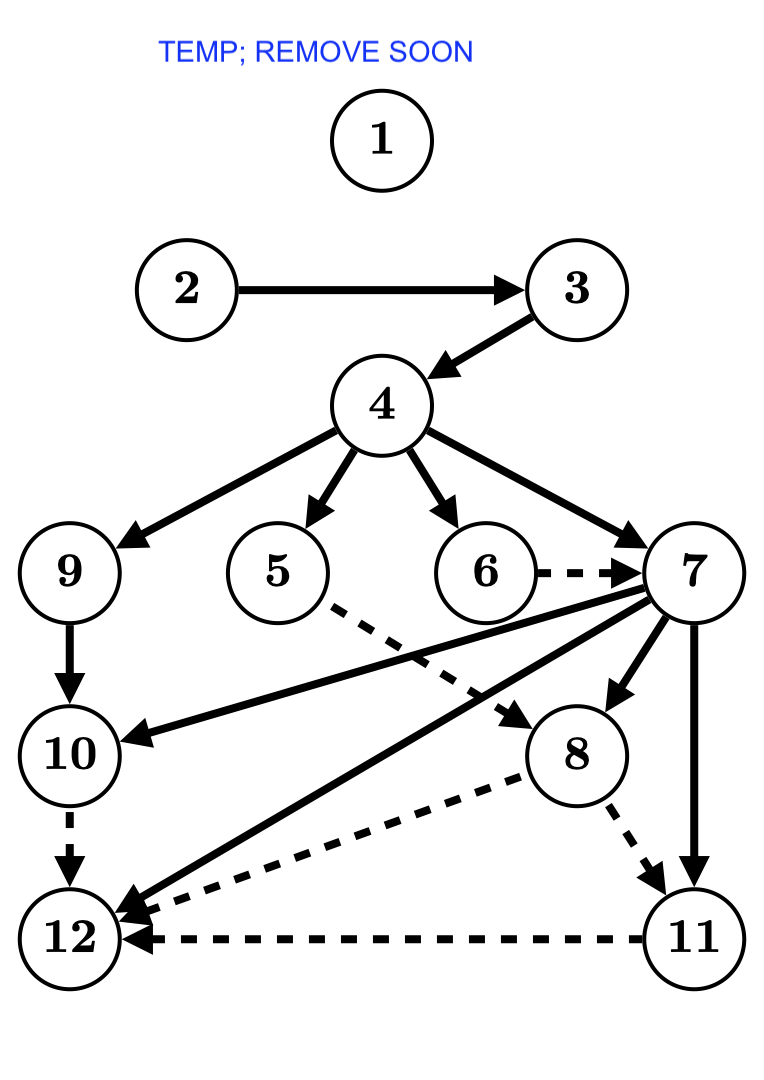
\includegraphics[width=\linewidth]{Interdependence.png}
    
    \newpage

    \textbf{Notes}:
    \interdependencenotes

    \mainmatter  % Now use arabic numerals for page numbers
}

%============= Index Pages ===============
\usepackage[
    totoc,
    columnsep=20pt,
    hangindent=8pt,
    subindent=20pt,
    subsubindent=30pt
]{idxlayout}

\makeindex[options= -s ../index-style.ist]

%======= Bibliography Formatting =========
% These two lines are here to ensure that URLs do not exceed the page by too much
\setcounter{biburllcpenalty}{7000}
\setcounter{biburlucpenalty}{8000}

\usepackage{xr}

\setasdraft  % TODO: Remove once no longer a draft

%=========== Global Variables ============
\newcommand{\version}{0.1}
\newcommand{\volumenumber}{2}
\newcommand{\volumename}{Rings}
\newcommand{\volumeimage}{cover/Integers Modulo n.png}

%============= Formatting ================
\linespread{1.05}

%============== Resources ================
\externaldocument{../Volume 0/Volume0}
\externaldocument{../Volume 1/Volume1}

%=========== Custom Commands =============
\newcommand{\ideal}[1]{\mathfrak{#1}}                % Ideal of a ring
\newcommand{\princ}[1]{\left\langle#1\right\rangle}  % Principal ideal generated by the element

\newcommand{\C}{\mathbb{C}}                        % The ring of complex numbers
\newcommand{\Mn}[2]{\mathcal{M}_{#1\times#1}(#2)}  % The ring of n by n matrices with entries in the ring R
\newcommand{\Q}{\mathbb{Q}}                        % The ring of rational numbers
\newcommand{\R}{\mathbb{R}}                        % The ring of real numbers
\newcommand{\Z}{\mathbb{Z}}                        % The ring of integers
\newcommand{\Zn}[1]{\mathbb{Z}_{#1}}               % The ring of integers modulo n

\newcommand{\Ann}[2]{\mathrm{Ann}_{#1}(#2)}  % Annihilator of a subset A of a ring R
\newcommand{\Char}[1]{\mathrm{char}(#1)}     % Characteristic of a ring R
\newcommand{\Nilr}[1]{\mathfrak{N}_{#1}}     % Nilradical of a ring R

%========= Front Matter Pages ============
% Quote page
\newcommand{\quotepagetext}{
    [Some] of the major discoveries in ring theory have helped shape the course of development of modern abstract algebra... A course in ring theory is an indispensable part of the education of any fledgling algebraist.
}
\newcommand{\quotepageattribution}{Tsit-Yuen Lam, 2001}
\newcommand{\quotepagecitation}{\cite{lam_2001}}

% Preface
\newcommand{\prefacevolumetext}{
    This volume covers the basics of ring theory. %TODO: Add
}
\newcommand{\prefacevolumedate}{}  %TODO: Add

% Suggestions of use
\newcommand{\interdependencenotes}{
    % TODO: Update
}

%=========================================
\begin{document}
\frontmatterpages

%=========================================
\chapter{Introduction to Rings}
In Volume I, we looked exclusively at groups and their operations. We discussed how groups are a generalisation of symmetry and looked at results related to groups. In this volume, we look at rings.

Before we introduce rings, we look at `simpler' algebraic structures and build our way up to them.

\section{Basic Algebraic Structures}
\begin{definition}
    A \textbf{magma}\index{magma} is a set $M$ together with a binary operation $\ast$ which is closed. That is, if $a$ and $b$ are in $M$, then $a \ast b \in M$. Such a magma is denoted $(M, \ast)$.
\end{definition}
\begin{example}
    Consider the set $M = \{1, 2, 3, 4\}$ with the operation $\ast$ such that $(M, \ast)$ has the Cayley table as shown below.
    \begin{table}[h]
        \centering
        \begin{tabular}{|l|l|l|l|l|}
            \hline
            $\ast$     & \textbf{1} & \textbf{2} & \textbf{3} & \textbf{4} \\ \hline
            \textbf{1} & 1          & 2          & 1          & 2          \\ \hline
            \textbf{2} & 2          & 3          & 4          & 1          \\ \hline
            \textbf{3} & 1          & 3          & 4          & 2          \\ \hline
            \textbf{4} & 2          & 1          & 2          & 1          \\ \hline
        \end{tabular}
    \end{table}
    
    Clearly for any $a, b\in M$ we have $a \ast b \in M$, so $(M, \ast)$ is a magma.
\end{example}

\begin{definition}
    A \textbf{semigroup}\index{semigroup} is a magma $(\mathcal{S}, \ast)$ where the operation $\ast$ is associative. That is, $a\ast(b\ast c) = (a\ast b)\ast c$.
\end{definition}
\begin{example}
    Consider the set $S = \{1, 2, 3, 4\}$ with the operation $\ast$ such that $(S, \ast)$ has the Cayley table as shown below.
    \begin{table}[h]
        \centering
        \begin{tabular}{|l|l|l|l|l|}
            \hline
            $\ast$     & \textbf{1} & \textbf{2} & \textbf{3} & \textbf{4} \\ \hline
            \textbf{1} & 1          & 1          & 1          & 1          \\ \hline
            \textbf{2} & 2          & 2          & 2          & 2          \\ \hline
            \textbf{3} & 3          & 3          & 3          & 3          \\ \hline
            \textbf{4} & 4          & 4          & 4          & 4          \\ \hline
        \end{tabular}
    \end{table}
    
    One sees that $(S, \ast)$ is closed under $\ast$. In addition, $\ast$ is associative. Hence $(S, \ast)$ is a semigroup.
\end{example}

\begin{definition}
    A \textbf{monoid}\index{monoid} is a semigroup $(M, \ast)$ with an element $e$, called the \textbf{identity}, such that
    \[
        e \ast m = m \ast e = m
    \]
    for all $m \in M$.
\end{definition}
\begin{example}
    Let $X$ be a set. Let the set
    \[
        S = \{f \vert  f: X \to X\}.
    \]
    and let $\circ$ denote function composition. Then $(S, \circ)$ forms a monoid:
    \begin{itemize}
        \item \textbf{Closure}: If $f, g \in S$ then $f\circ g \in S$ since function composition is closed.
        \item \textbf{Associative}: Function composition is associative.
        \item \textbf{Identity}: The identity function $\id: X \to X, x\mapsto x$ is inside $S$ and
        \[
            \id \circ f = f \circ \id = f
        \]
        for all $f \in S$.
    \end{itemize}
    Thus $(S, \circ)$ forms a monoid.
\end{example}

\begin{definition}
    A \textbf{group}\index{group} is a monoid $(G, \ast)$ where every element has an inverse. That is to say, for every $g \in G$, there exists $g^{-1} \in G$ such that
    \[
        g \ast g^{-1} = g^{-1} \ast g = e
    \]
    where $e$ is the identity in $G$.
\end{definition}

\section{Definition of a Ring}
With all that setup, we are ready to define what a ring is. Note that we follow \cite[p.~223]{dummit_foote_2004}, \cite[p.~115, Definition 1.1]{hungerford_1980}, and \cite{proofwiki_ringdefinition} for the definition of a ring.
\begin{definition}
    A \textbf{ring}\index{ring} is a set $R$ with two binary operations $+$ and $\cdot$ satisfying the following axioms.
    \begin{itemize}
        \item \textbf{Addition-Abelian}: $(R, +)$ is an abelian group.
        \item \textbf{Multiplication-Semigroup}: $(R, \cdot)$ is a semigroup.
        \item \textbf{Distributive}: $\cdot$ is distributive over $+$. That is,
        \begin{itemize}
            \item $a \cdot (b + c) = (a \cdot b) + (b \cdot c)$; and
            \item $(a + b) \cdot c = (a \cdot c) + (b \cdot c)$.
        \end{itemize}
    \end{itemize}
    One may denote such a ring by $(R, +, \cdot)$.
\end{definition}
\begin{remark}
    Other authors (e.g. \cite[p.~136]{cohn_1982}, \cite[pp.~145--146]{clark_1984}) may require that $(R, \cdot)$ is a monoid. In this book, any ring that satisfies the above condition is called a \textbf{ring with identity}\index{ring!with identity}.
\end{remark}
\begin{remark}
    A ring where $a \cdot b = b \cdot a$ for all $a$ and $b$ in $R$ is called a \textbf{commutative ring}\index{ring!commutative}.
\end{remark}

We end this chapter by introducing the \textbf{trivial ring}.
\begin{definition}
    The \textbf{trivial ring}\index{trivial ring} (or \textbf{zero ring}\index{zero ring}), denoted $\textbf{0}$, is the ring $(\{0\}, +, \cdot)$ where
    \[
        0 + 0 = 0 \text{ and } 0 \cdot 0 = 0.    
    \]
\end{definition}
\begin{exercise}
    Prove that the trivial ring is a commutative ring with identity.
\end{exercise}

%=========================================
\chapter{Basics of Rings}
With basic algebraic structures and the definition of a ring out of the way, we are now ready to tackle the basics of rings in this chapter.

\section{Basic Examples of Rings}
Before we introduce some examples of rings, we make some remarks for the notation that is used in Ring Theory.
\begin{itemize}
    \item The multiplication symbol $\cdot$ is usually omitted, so $x \cdot y$ is written as $xy$.
    \item The additive identity of $R$ will always be denoted by 0 and the multiplicative identity of $R$ (if it exists) will always be denoted by 1.
    \item The additive inverse of the element $x$ will be denoted by $-x$ and the multiplicative inverse of $x$ (if it exists) will be denoted by $x^{-1}$.
    \item $n$ applications of $+$ on an element $x$ will be denoted $nx$ (and will be denoted $-nx$ if the element is $-x$), while $n$ applications of $\cdot$ on an element $x$ will be denoted $x^n$ (and will be denoted $x^{-n}$ if the element is $x^{-1}$ and if it exists).
\end{itemize}

Let's look at some examples of rings.
\begin{example}
    We show that $(\Zn{n}, \oplus_n, \otimes_n)$, where $\oplus_n$ and $\otimes_n$ denote addition and multiplication modulo $n$ respectively, form a ring.
    \begin{itemize}
        \item \textbf{Addition-Abelian}: We know $(\Zn{n}, \oplus_n)$ is an abelian group from Volume I.
        \item \textbf{Multiplication-Semigroup}: We can see that $(\Zn{n}, \otimes_n)$ is a semigroup as
        \begin{itemize}
            \item $\Zn{n}$ is closed under $\otimes_n$ because $a \otimes_n b \in \{0, 1, 2, \dots, n-1\} = \Zn{n}$; and
            \item multiplication is associative, so multiplication modulo $n$ is associative.
        \end{itemize}
        \item \textbf{Distributive}: It is clear that $\oplus_n$ and $\otimes_n$ distribute.
    \end{itemize}
    Hence $(\Zn{n}, \oplus_n, \otimes_n)$ is a ring. Furthermore, $\otimes_n$ has an identity of 1 and is commutative, so in fact $(\Zn{n}, \otimes_n)$ is a commutative monoid. Therefore $(\Zn{n}, \oplus_n, \otimes_n)$ is a commutative ring with identity.

    Note that, in this volume, $\Zn{n}$ refers to the ring $(\Zn{n}, \oplus_n, \otimes_n)$.
\end{example}

\begin{example}
    We show that $(\Q, +, \times)$, where $+$ and $\times$ denote normal addition and multiplication, form a ring.
    \begin{itemize}
        \item \textbf{Addition-Abelian}: From Volume I, we know that $(\Q, +)$ is an abelian group.
        \item \textbf{Multiplication-Semigroup}: We note that $(\Q, \times)$ is a semigroup as
        \begin{itemize}
            \item $Q$ is closed under $\times$ because multiplying two rational numbers together produce a rational number; and
            \item multiplication is associative.
        \end{itemize}
        \item \textbf{Distributive}: It is clear that $+$ and $\times$ distribute.
    \end{itemize}
    Hence $(\Q, +, \times)$ is a ring. Furthermore, $\times$ has an identity of 1 and is commutative. So, just like $\Zn{n}$, we see that $(\Q, +, \times)$ is a commutative ring with identity.

    Note that, in this volume, $\Q$ refers to the ring $(\Q, +, \times)$.
\end{example}

\begin{exercise}
    Prove that $\Z$ is a ring under regular addition and multiplication.\newline
    (\textit{You do \textbf{not} need to prove the \textbf{Distributive} axiom.})
\end{exercise}
Note that, in this volume, $\Z$ refers to the ring $(\Z, +, \times)$.

We remark that both $\R$ and $\C$ are rings under regular addition and multiplication, although we will not prove it here.

We look at one more ring: the ring of $n \times n$ matrices.

Let $\Mn{n}{R}$ denote the set of $n\times n$ matrices with entries in the ring $(R, \oplus, \otimes)$.
\begin{itemize}
    \item We define \textbf{matrix addition}\index{matrix addition} within this set. Suppose we have $\textbf{A}, \textbf{B} \in \Mn{n}{R}$, and let their sum be $\textbf{C} = \textbf{A} + \textbf{B}$. Then
    \[
        c_{i,j} = a_{i,j} \oplus b_{i,j}    
    \]
    where $\oplus$ is the addition operation in the ring $R$.
    
    \item We define \textbf{matrix multiplication}\index{matrix multiplication} within this set. Suppose $\textbf{A}, \textbf{B} \in \Mn{n}{R}$, and let their product be $\textbf{C} = \textbf{AB}$. Then
    \begin{align*}
        c_{i,j} &= (a_{i,1}\otimes b_{1,j}) \oplus (a_{i,2}\otimes b_{2,j}) \oplus \cdots \oplus (a_{i,n}\otimes b_{n,j})\\
        &= \sum_{k=1}^n (a_{i,k}\otimes b_{i,k})
    \end{align*}
    where $\oplus$ and $\otimes$ are the addition and multiplication operations in the ring $R$ respectively.
\end{itemize}

\begin{proposition}
    $\Mn{n}{R}$ is a ring under matrix addition and matrix multiplication.
\end{proposition}
\begin{proof}
    We need to prove that the ring axioms hold.
    \begin{itemize}
        \item \textbf{Addition-Abelian}: We first prove that $(\Mn{n}{R}, +)$ is indeed an abelian group.
        \begin{itemize}
            \item \textbf{Closure}: Clearly the sum of any two matrices in $\Mn{n}{R}$ is also a square matrix with $n$ rows with elements inside $R$, meaning that $\Mn{n}{R}$ is closed under matrix addition.

            \item \textbf{Associative}: Let the matrices $\textbf{A}$, $\textbf{B}$, and $\textbf{C}$ belong inside $\Mn{n}{R}$. Let $\textbf{P} = \textbf{A} + (\textbf{B} + \textbf{C})$ and $\textbf{Q} = (\textbf{A} + \textbf{B}) + \textbf{C}$. We note that $\textbf{P} = \textbf{Q}$ as
            \begin{align*}
                p_{i,j} &= a_{i,j} \oplus (b_{i,j} \oplus c_{i,j})\\
                &= (a_{i,j} \oplus b_{i,j}) \oplus c_{i,j} & (\oplus\text{ is associative})\\
                &= q_{i,j}
            \end{align*}
            which proves that matrix addition is associative.
    
            \item \textbf{Identity}: Denote the $n \times n$ matrix with contains only the zero in $R$ by $\textbf{0}_n$. One sees clearly that this is the identity in $\Mn{n}{R}$ as $\textbf{M} + \textbf{0}_n = \textbf{M}$ for any matrix in $\Mn{n}{R}$.
            
            \item \textbf{Inverse}: Let $\textbf{A} \in \Mn{n}{R}$. Define the matrix $\textbf{B} = -\textbf{A}$ where
            \[
                b_{i,j} = -a_{i,j},    
            \]
            that is, $b_{i,j}$ contains the additive inverse of $a_{i,j}$ in the ring $R$. Then one sees that $\textbf{A} + \textbf{B} = \textbf{0}_n$.\newline
            (Note that we denote the additive inverse of a matrix $\textbf{M}$ by $-\textbf{M}$.)

            \item \textbf{Commutative}: Let $\textbf{A}, \textbf{B} \in \Mn{n}{R}$. Set $\textbf{C} = \textbf{A} + \textbf{B}$ and $\textbf{D} = \textbf{B} + \textbf{C}$. Then
            \begin{align*}
                c_{i,j} &= a_{i,j} \oplus b_{i,j}\\
                &= b_{i,j} \oplus a_{i,j} & (\oplus \text{ is commutative})\\
                &= d_{i,j}
            \end{align*}
            which means $\textbf{C} = \textbf{D}$.
        \end{itemize}

        \item \textbf{Multiplication-Semigroup}: We now need to prove that $(\Mn{n}{R}, \cdot)$ is a semigroup.
        \begin{itemize}
            \item \textbf{Closure}: In Volume I we showed that matrix multiplication produces another $n \times n$ matrix. Furthermore the entries of the new matrix are elements of $R$. Hence $\Mn{n}{R}$ is closed under matrix multiplication.
        
            \item \textbf{Associative}: We proved matrix multiplication is associative in Volume I.
        \end{itemize}
        
        \item \textbf{Distributive}: We prove only $\textbf{A}(\textbf{B} + \textbf{C}) = (\textbf{AB}) + (\textbf{AC})$ as the other case is proven similarly.
        
        Let $\textbf{R} = \textbf{A}(\textbf{B} + \textbf{C})$, $\textbf{G} = \textbf{AB}$, and $\textbf{H} = \textbf{AC}$. We note
        \begin{align*}
            r_{i,j} &= \sum_{k=1}^n \left(a_{i,k} \otimes \left(b_{k,j} \oplus c_{k,j}\right)\right)\\
            &= \sum_{k=1}^n \left((a_{i,k} \otimes b_{k,j}) \oplus (a_{i,k} \otimes c_{k,j})\right)\\
            &= \left(\sum_{k=1}^n (a_{i,k} \otimes b_{k,j})\right) \oplus \left(\sum_{k=1}^n (a_{i,k} \otimes c_{k,j})\right)\\
            &= g_{i,j}\oplus h_{i,j}
        \end{align*}
        which means $\textbf{R} = \textbf{G} + \textbf{H}$.
    \end{itemize}
    As all the ring axioms are satisfied, thus $\Mn{n}{R}$ is a ring.
\end{proof}
For brevity, we let $\Mn{n}{R}$ denote the ring under matrix addition and multiplication.

\section{General Properties of Rings}
We list some properties of rings here. For each of the propositions, assume $R$ is a ring.

\begin{proposition}\label{prop-multiplying-by-zero-is-zero}
    $0x = x0 = 0$ for all $x \in R$.
\end{proposition}
\begin{proof}
    We note that
    \begin{align*}
        0x &= (0 + 0)x & (0 \text{ is additive inverse})\\
        &= 0x + 0x & (\text{by \textbf{Distributive} axiom})
    \end{align*}
    so by `subtracting' $0x$ on both sides (i.e., adding $-0x$ on both sides) we see $0 = 0x$. A similar argument shows that $x0 = 0$.
\end{proof}

\begin{proposition}\label{prop-product-of-element-and-additive-inverse-is-additive-inverse-of-product}
    $(-a)b = a(-b) = -(ab)$ for any $a$ and $b$ in $R$.
\end{proposition}
\begin{proof}
    We show that $(-a)b = -(ab)$ and $a(-b) = -(ab)$ to complete the proof.
    \begin{itemize}
        \item Note $(-a)b + ab = (-a + a)b = 0b = 0$ by \textbf{Distributive} axiom. Hence by subtracting $ab$ on both sides we see $(-a)b = -(ab)$.
        \item Note also $a(-b) + ab = a(-b + b) = a0 = 0$ by \textbf{Distributive} axiom. Hence by subtracting $ab$ on both sides we see $a(-b) = -(ab)$.
    \end{itemize}
    Result follows.
\end{proof}

\begin{proposition}
    $(-a)(-b) = ab$ for any $a$ and $b$ in $R$.
\end{proposition}
\begin{proof}
    See \myref{exercise-product-of-additive-inverses} (later).
\end{proof}

\begin{proposition}
    If $R$ has an identity, it is unique.
\end{proposition}
\begin{proof}
    Suppose 1 and $1'$ are identities, and consider the sum $1 + 1'$. Then
    \begin{align*}
        1 + 1' &= 1'(1+1') & (\text{multiplying by identity }1')\\
        &= 1'1 + 1'1' & (\text{by \textbf{Distributive} axiom})\\
        &= 1' + 1'. & (1 \text{ and } 1' \text{ are identities})
    \end{align*}
    Subtracting $1'$ on both sides yields $1 = 1'$, meaning that the identity is unique.
\end{proof}

\begin{exercise}\label{exercise-product-of-additive-inverses}
    Show that $(-a)(-b) = ab$ for any $a$ and $b$ in $R$.
\end{exercise}

\section{More Definitions}
Suppose $R$ is a ring.
\begin{definition}
    We say that $a \neq 0$ is a \textbf{zero divisor}\index{zero divisor} if there exists $b \neq 0$ such that $ab = 0$.
\end{definition}
\begin{example}
    Consider the ring $\Zn{12}$. Clearly 4 and 6 are in $\Zn{12}$, and their product is $24 = 2 \times 12 = 0$ in $\Zn{12}$. Hence 4 and 6 are zero divisors in $\Zn{12}$.
\end{example}
\begin{example}
    We claim that the ring
    \[
        R = \{f: [0, 1] \to [0, 1]\}
    \]
    has zero divisors. Consider the functions
    \begin{align*}
        f(x) &= x\\
        g(x) &= \begin{cases}
            0 & \text{ if } x \neq 0\\
            1 & \text{ if } x = 0
        \end{cases}
    \end{align*}
    Clearly neither of them are the zero function. However, consider $f(x)g(x)$.
    \begin{itemize}
        \item If $x \neq 0$, then $g(x) = 0$ which means $f(x)g(x) = 0$.
        \item If $x = 0$, then $f(x) = 0$ which means $f(x)g(x) = 0$.
    \end{itemize}
    Hence their product is the zero function, meaning that $R$ has zero divisors $f$ and $g$.
\end{example}
\begin{exercise}
    Does the ring $\Mn{2}{\mathbb{R}}$ have zero divisors?
\end{exercise}
We note one property about zero divisors, which will be used in future chapters.
\begin{proposition}\label{prop-zero-divisors-have-no-inverses}
    Zero divisors do not have inverses.
\end{proposition}
\begin{proof}
    Assume $a \neq 0$ and $b \neq 0$ are zero divisors in the ring $R$, so $ab = 0$. Seeking a contradiction, assume $a$ has an inverse, so
    \[
        b = (a^{-1}a)b = a^{-1}(ab) = a^{-1}0 = 0    
    \]
    which contradicts $b \neq 0$. Hence a zero divisor has no inverse.
\end{proof}

\begin{definition}
    Suppose $0 \neq 1$. An element $u \in R$ is called a \textbf{unit}\index{unit} if there exists a $v \in R$ such that $uv=vu=1$. Equivalently, $u$ is a unit if it has a multiplicative inverse.
\end{definition}
\begin{example}
    3 and 7 are units in $\Zn{10}$ since $3 \times 7 = 7 \times 3 = 21 = 1$ in $\Zn{10}$.
\end{example}

\begin{definition}
    If every non-zero element $x \in R$ is a unit, then $R$ is said to be a \textbf{division ring}\index{division ring}.
\end{definition}
\begin{remark}
    A division ring is a ring with identity since every element is a unit in a division ring.
\end{remark}

\begin{definition}
    A commutative division ring where $0 \neq 1$ is called a \textbf{field}\index{field}.
\end{definition}
We look at fields in more detail in Volume III.

\begin{exercise}\label{exercise-Z-is-not-a-field}
    Is $\Z$ a field?
\end{exercise}

\section{Subrings}
We end this chapter off with an exploration about subrings.

\begin{definition}
    Let $R$ be a ring and $S$ be a subset of $R$. Then $S$ is a \textbf{subring}\index{subring} of $R$ if
    \begin{itemize}
        \item $(S, +) \leq (R, +)$, i.e. the set $S$ under addition is a subgroup of $R$ under addition; and
        \item For all $a$ and $b$ in $S$ we have $ab \in S$, i.e. $S$ is closed under multiplication.
    \end{itemize}
\end{definition}
\begin{remark}
    Alternatively, one may show that $S$ is a ring to prove that $S$ is a subring of $R$.
\end{remark}

\begin{example}
    We know that $\Z$ and $\Q$ are rings, and clearly $\Z \subseteq \Q$. Hence $\Z$ is a subring of $\Q$. Similarly, $\Q$ is a subring of $\R$, and $\R$ is a subring of $\C$.
\end{example}

\begin{example}
    Consider the \textbf{gaussian integers}\index{gaussian integers},
    \[
        \Z[i] = \{a + bi \vert a,b\in\mathbb{Z}\},
    \]
    where $i$ is the imaginary unit (i.e., $i^2 = -1$). We will show that $\Z[i]$ is a subring of $\C$.
    \begin{proof}
        Clearly $\Z[i] \subseteq \C$. We show that $(\Z[i], +) \leq (\C, +)$.
        \begin{itemize}
            \item Clearly the identity of $(\C, +)$, which is 0, is inside $(\Z[i], +)$ as $0 = 0 + 0i$.
            \item For any $a + bi, c+di \in \Z[i]$, we have $(a+bi) + (-(c+di)) = (a-c) + (b-d)i \in \Z[i]$.
        \end{itemize}
        Therefore by subgroup test we see $(\Z[i], +) \leq (\C, +)$.

        Now we show that $\Z[i]$ is closed under multiplication. Let $a + bi, c+di \in \Z[i]$. Then their product is
        \begin{align*}
            (a+bi)(c+di) &= ac+adi+bci+bdi^2\\
            &= (ac-bd) + (ad+bc)i
            &\in \Z[i]
        \end{align*}
        so $\Z[i]$ is closed under multiplication. Therefore $\Z[i]$ is a subring of $\C$.
    \end{proof}
\end{example}
\begin{exercise}
    Show that
    \[
        R = \left\{\begin{pmatrix}a&a\\a&a\end{pmatrix} \vert a \in \R\right\}
    \]
    is a subring of $\Mn{2}{\mathbb{R}}$.
\end{exercise}

\newpage

\section{Problems}
\begin{problem}
    Let $R$ be a ring. Prove that if $u \in R$ is a unit then so is $-u$.
\end{problem}

\begin{problem}
    Prove that the trivial ring is the unique ring with identity in which $0 = 1$.
\end{problem}

\begin{problem}
    Let $(R, \ast)$ be a magma. If $(R, \ast, \ast)$ is a ring, describe the elements in $R$.
\end{problem}

\begin{problem}
    Prove that it is impossible for an element of a ring $R$ to be both a zero divisor and a unit.
\end{problem}

\begin{problem}
    Show that
    \[
        \Q[\sqrt2] = \{a + b\sqrt2 \vert a,b \in \Q\}
    \]
    is a ring. Hence show it is a field.
\end{problem}

\begin{problem}
    Let
    \[
        R = \left\{\begin{pmatrix}a&b\\0&0\end{pmatrix} \vert a,b \in \R\right\}    
    \]
    be a ring under matrix addition and multiplication.
    \begin{enumerate}[label=(\roman*)]
        \item Show that $R$ has no identity.
        \item Show that $R$ contains a non-trivial subring $S$ with identity.
    \end{enumerate}
\end{problem}

\begin{problem}
    A ring $R$ is called a \textbf{Boolean ring}\index{Boolean ring} if $r^2 = r$ for all $r \in R$.
    \begin{enumerate}[label=(\roman*)]
        \item Show that $r = -r$ for all $r \in R$.
        \item Prove that every Boolean ring is commutative.
    \end{enumerate}
\end{problem}

\begin{problem}
    Let $R$ be a commutative ring with identity. We say that an element $x$ in $R$ is \textbf{nilpotent}\index{nilpotent} if there exists a positive integer $n$ such that $x^n = 0$.
    \begin{enumerate}[label=(\roman*)]
        \item Show that the product of two units is a unit.
        \item Let $u \in R$ be a unit and $x \in R$ be nilpotent. Show that $ux$ is nilpotent.
        \item Show that $u - x$ is a unit.
    \end{enumerate}
\end{problem}

%=========================================
\chapter{Integral Domains}
We explored the absolute basics of rings in the previous chapter. When working in abstract algebra, we usually prefer rings with slightly more structure as they allow us to generate more useful and applicable results. Integral domains are an important category of rings, which we explore in this chapter.

\section{Definition and Examples}
\begin{definition}
    An \textbf{integral domain}\index{integral domain} is a commutative ring with identity and no zero divisors.
\end{definition}
Recall that an element $a \neq 0$ is a zero divisor if there exists a $b \neq 0$ such that $ab = 0$. What we mean is that an integral domain has no such element.

\begin{example}
    We show that the ring $\Z$ is an integral domain. We note that $\Z$ is a commutative ring as multiplication is commutative. Furthermore, clearly 1 is the multiplicative identity in $\Z$. All that remains is to show that there does not exist any zero divisors.

    Suppose $a$ and $b$ are non-zero elements in $\Z$. We show that $ab \neq 0$ to prove that there does not exist any zero divisors. Let's first consider the case when $b > 0$. Then we may write
    \[
        ab = \underbrace{a + a + \cdots + a}_{b \text{ times}}
    \]
    which clearly is not zero since $a \neq 0$. Now if $b < 0$ then note
    \[
        ab = (-a)(-b) = \underbrace{(-a) + (-a) + \cdots + (-a)}_{(-b) \text{times}}
    \]
    which is also not zero as $-a \neq 0$. Hence there are no zero divisors in $\Z$.

    Therefore $\Z$ is an integral domain.
\end{example}
\begin{example}
    We show that the ring $\Z[i]$, the gaussian integers, is an integral domain. Similar to $\Z$, we note multiplication is commutative with identity 1.

    Suppose $w$ and $z$ are non-zero elements in $\Z[i]$; write $w = a+bi$ and $z = c+di$. Note that $a^2+b^2 \neq 0$ and $c^2 + d^2 \neq 0$. Now clearly
    \[
        wz = (a+bi)(c+di) = ac+adi+bci+bdi^2 = (ac-bd) + (ad+bc)i
    \]
    and
    \begin{align*}
        (ac-bd)^2 + (ad+bc)^2 &= (a^2c^2 - 2abcd + b^2d^2) +\\
        &\quad(a^2d^2 + 2abcd + b^2c^2)\\
        &= a^2c^2 + a^2d^2 + b^2c^2 + b^2d^2\\
        &= (a^2 + b^2)(c^2 + d^2)\\
        &\neq 0
    \end{align*}
    which hence means that $wz \neq 0$. Therefore $\Z[i]$ has no zero divisors, thereby meaning that $\Z[i]$ is indeed an integral domain.
\end{example}

We note an interesting result regarding fields here.
\begin{proposition}\label{prop-field-is-integral-domain}
    Any field is an integral domain.
\end{proposition}
\begin{proof}
    Any non-zero element in a field is a unit, i.e. has an inverse. Now by \myref{prop-zero-divisors-have-no-inverses}, any zero divisor must not have an inverse; the converse being that any element that has an inverse cannot be a zero divisor. Hence, there are no zero divisors in a field. Now a field is commutative, therefore meaning that the field is an integral domain.
\end{proof}

Let's look at some non-examples of integral domains.
\begin{example}
    The ring $\Mn{n}{R}$ where $R$ is any ring is not an integral domain since $\Mn{n}{R}$ is not commutative.
\end{example}
\begin{example}
    The ring $2\Z$ is not an integral domain as it does not contain a multiplicative identity (namely, 1).
\end{example}
\begin{example}
    The ring $\Z \times \Z$ under pairwise addition and multiplication is not an integral domain as $(0,1) \neq (0, 0)$ and $(1, 0) \neq (0, 0)$ but $(0,1)(1,0) = (0, 0)$, meaning that $\Z \times \Z$ contains a zero divisor.
\end{example}

\begin{exercise}
    Prove that the ring
    \[
        \Z[\sqrt2] = \left\{a + b\sqrt2 \vert a,b \in \Z\right\}
    \]
    is an integral domain.
\end{exercise}
\begin{exercise}
    Explain why all $\Zn{n}$ where $n$ is a positive composite number are not integral domains.
\end{exercise}

\section{General Results}
With an introduction of integral domains out of the way, we introduce some general results applicable to integral domains.
\begin{proposition}[Cancellation Law]\index{integral domain!cancellation law}
    Let $R$ be an integral domain, $r, x, y \in R$, and $r \neq 0$. Then the following statements are equivalent.
    \begin{enumerate}[label=(\arabic*)]
        \item $x = y$
        \item $rx = ry$
        \item $xr = yr$
    \end{enumerate}
\end{proposition}
\begin{proof}
    We prove the statements in order.
    \begin{itemize}
        \item $\boxed{(1) \implies (2)}$ Given $x = y$, this means $x - y = 0$. Multiplying $r$ on the left on both sides yields $r(x-y) = r0 = 0$. Distributing yields $rx - ry = 0$ which hence means $rx = ry$.
        
        \item $\boxed{(2) \implies (3)}$ Given $rx = ry$. Multiplying $r$ on the right on both sides yields $rxr = ryr$, thereby meaning $rxr - ryr = 0$. Factoring yields $r(xr - yr) = 0$. As $R$ is an integral domain, the only way for this to occur is if $r = 0$ (which is impossible) or $xr - yr = 0$. Therefore $xr = yr$.
        
        \item $\boxed{(3) \implies (1)}$ Given $xr = yr$ we may write $xr - yr = (x-y)r = 0$. Since $R$ is an integral domain we must have $x - y = 0$ or $r = 0$ (impossible as $r \neq 0$). Hence $x = y$.
    \end{itemize}
    This proves the proposition.
\end{proof}

\newpage

\begin{theorem}\label{thrm-finite-integral-domain-is-field}
    Every finite integral domain is a field.
\end{theorem}
\begin{proof}
    A finite integral domain is a commutative ring with identity; all that remains is to prove that every non-zero element has an inverse.

    Suppose $R$ is a finite integral domain and take a non-zero element $r$ in $R$. Consider the set
    \begin{align*}
        A &= \{r^k \vert k \in \Z,\;k\geq 0\}\\
        &= \{1, r, r^2, r^3, \dots\}\\
        &\subseteq R.
    \end{align*}
    Note that as $R$ is finite we must have $A$ be finite as well. Therefore there must exist positive integers $m$ and $n$ with $m > n$ such that $r^m = r^n$, meaning $r^m - r^n = 0$. As $m > n$, thus $r^n\left(r^{m-n}-1\right) = 0$. Hence either $r^n = 0$ or $r^{m-n} - 1 = 0$.

    Now if $r^n = 0$ then $n > 1$ (since $r^1 = r \neq 0$ by assumption). Note $r^n = rr^{n-1} = 0$, which hence means $r^{n-1} = 0$ as $r \neq 0$ and $R$ has no zero divisors. But we may repeat this argument on $n - 1$ to eventually terminate at $r = 0$, which is a contradiction. Hence we must conclude that $r^{m-n} - 1 = 0$. We may write $r^{m-n}-1 = 0$ as $rr^{m-n-1} = 1$ which means that $r$ is a unit (as $r^{m-n-1}$ is its inverse). Therefore every non-zero element has an inverse.

    Hence $R$ is a field.
\end{proof}

\begin{remark}
    We note that finite fields are also known as \textbf{Galois fields}\index{Galois Field}, so-named in honour of \'{E}variste Galois. We explore more properties of fields and Galois fields in Volume III.
\end{remark}

\begin{example}
    Let $p$ be a prime and consider the ring $\Zn{p}$. Clearly multiplication is commutative with identity 1. Also, as the only way to factor $p$ is $1 \times p$ and since $p \notin \Zn{p}$, thus there are no zero divisors in $\Zn{p}$. Hence $\Zn{p}$ is an integral domain. Now $\Zn{p}$ only has $p$ elements (namely the integers 0 to $p - 1$), so it is finite. By \myref{thrm-finite-integral-domain-is-field} we know that $\Zn{p}$ is a field.
\end{example}

\begin{example}
    We show that $\Zn{3}[i] = \{a+bi \vert a,b \in \Zn{3}\}$ is a finite integral domain in order to show that it is a field. Clearly multiplication is commutative with identity 1, so we just need to show that there are no zero divisors in $\Zn{3}[i]$.
    \begin{table}[h]
        \centering
        \resizebox{\textwidth}{!}{
            \begin{tabular}{|l|l|l|l|l|l|l|l|l|}
            \hline
            $\boldsymbol{\times}$ & $\boldsymbol{1}$ & $\boldsymbol{2}$ & $\boldsymbol{i}$ & $\boldsymbol{1+i}$ & $\boldsymbol{2+i}$ & $\boldsymbol{2i}$ & $\boldsymbol{1+2i}$ & $\boldsymbol{2+2i}$ \\ \hline
            $\boldsymbol{1}$    & 1      & 2      & $i$    & $1+i$  & $2+i$  & $2i$   & $1+2i$ & $2+2i$ \\ \hline
            $\boldsymbol{2}$    & 2      & 1      & $2i$   & $2+2i$ & $1+2i$ & $i$    & $2+i$  & $1+i$  \\ \hline
            $\boldsymbol{i}$    & $i$    & $2i$   & 2      & $2+i$  & $2+2i$ & 1      & $1+i$  & $1+2i$ \\ \hline
            $\boldsymbol{1+i}$  & $1+i$  & $2+2i$ & $2+i$  & $2i$   & 1      & $1+2i$ & 2      & $i$    \\ \hline
            $\boldsymbol{2+i}$  & $2+i$  & $1+2i$ & $2+2i$ & 1      & $i$    & $1+i$  & $2i$   & 2      \\ \hline
            $\boldsymbol{2i}$   & $2i$   & $i$    & 1      & $1+2i$ & $1+i$  & 2      & $2+2i$ & $2+i$  \\ \hline
            $\boldsymbol{1+2i}$ & $1+2i$ & $2+i$  & $1+i$  & 2      & $2i$   & $2+2i$ & $i$    & 1      \\ \hline
            $\boldsymbol{2+2i}$ & $2+2i$ & $1+i$  & $1+2i$ & $i$    & 2      & $2+i$  & 1      & $2i$   \\ \hline
            \end{tabular}
        }
    \end{table}
    
    From the table, we have shown that no two non-zero elements in $\Zn{3}[i]$ multiply to zero. Therefore $\Zn{3}[i]$ has no zero divisors, which means $\Zn{3}[i]$ is an integral domain. Furthermore, as $\Zn{3}[i]$ is finite, therefore we know that it is a finite field by \myref{thrm-finite-integral-domain-is-field}.
\end{example}

\begin{exercise}\label{exercise-Zn2[alpha]}
    Is the ring
    \[
        \Zn{2}[\alpha] = \{a+b\alpha \vert a,b\in\Zn{2}\}
    \]
    where $\alpha^2 = 1 + \alpha$ under regular addition and multiplication a field?
\end{exercise}

\section{Characteristic of a Ring}
\begin{definition}
    Let $R$ be a ring. We say that \textbf{characteristic}\index{characteristic} of $R$ is $n$ if $n$ is the smallest positive integer such that
    \[
        nr = \underbrace{r+r+\cdots+r}_{n \text{ times}} = 0
    \]
    for all $r \in R$. We then write $\Char{R} = n$. If no such $n$ exists we say $\Char{R} = 0$.
\end{definition}

We look at two properties about the characteristic.
\begin{proposition}
    If $R$ is a ring with identity and $\Char{R} \neq 0$, then $\Char{R}$ is equal to the order of 1 in the group $(R, +)$.
\end{proposition}
\begin{proof}
    Let $\Char{R} = n$ and the order of 1 in the group $(R, +)$ be $m$. Our goal is to show that $m = n$.

    On one hand, note that
    \[
        n1 = \underbrace{1+1+1+\cdots+1}_{n \text{ times}} = 0
    \]
    by definition of the characteristic of a ring. Note also that $m1 = \underbrace{1+1+1+\cdots+1}_{m \text{ times}} = 0$ by definition of the order of an element in the group $(R, +)$. By \myref{problem-element-to-power-of-multiple-of-order-is-identity}, this means that $n$ is a multiple of $m$, which thus means $m \leq n$.

    On another hand, for any $r \in R$, we know that
    \begin{align*}
        \underbrace{r + r + r + \cdots + r}_{m \text{ times}} &= r(\underbrace{1+1+1+\cdots+1}_{m \text{ times}})\\
        &= r0 & (|1| = m \text{ in } (R,+))\\
        &= 0.
    \end{align*}
    The minimality of the characteristic $n$ means that $m$ has to be at least $n$, i.e. $m \geq n$.

    Since $m \leq n$ and $m \geq n$, thus $m = n$.
\end{proof}

\begin{proposition}\label{prop-zero-of-prime-characteristic-if-integral-domain}
    If $R$ is an integral domain, then either $\Char{R} = 0$ or $\Char{R} = p$ where $p$ is a prime.
\end{proposition}
\begin{proof}
    If $\Char{R} = 0$ we are done, so assume that $\Char{R} = n \neq 0$. Furthermore assume $n = ab$ with $1 \leq a,b \leq n$.

    Note that
    \[
        0 = \underbrace{1 + 1 + \cdots + 1}_{n \text{ times}} = (\underbrace{1+1+\cdots+1}_{a \text{ times}})(\underbrace{1+1+\cdots+1}_{b \text{ times}}).
    \]
    As $R$ is an integral domain, this means that either
    \[
        \underbrace{1+1+\cdots+1}_{a \text{ times}} = 0 \text{ or } \underbrace{1+1+\cdots+1}_{b \text{ times}} = 0.
    \]
    Without loss of generality, assume that $\underbrace{1+1+\cdots+1}_{a \text{ times}} = 0$. By the minimality of $\Char{R} = n$, this means that $a \geq n$. But we assumed that $a \leq n$, so we must have $a = n$. Therefore $a = n$ and $b = 1$ which is exactly what we need to show that $n$ is a prime.
\end{proof}

\begin{exercise}\label{exercise-trivial-ring-is-not-an-integral-domain}
    Is the trivial ring an integral domain?
\end{exercise}
\begin{exercise}
    What is the characteristic of the ring $\Zn2[\alpha]$ (as defined in \myref{exercise-Zn2[alpha]})?
\end{exercise}

\section{Links to Polynomial Rings}
We end this chapter off with introducing a theorem that provides a condition for when a ring is an integral domain. Before that, let's look at polynomial rings.
\begin{definition}
    Let $R$ be a ring and $x$ be an indeterminate (i.e., variable). Then the \textbf{polynomial ring}\index{polynomial ring} $R[x]$ is the set of all polynomials with coefficients in $R$. That is,
    \[
        R[x] = \left\{a_0+a_1x+a_2x^2+\cdots+a_nx^n \vert n \in \mathbb{N}\cup\{0\},\;a_i \in R\right\}.
    \]
    It should be noted that any polynomial in $R[x]$ has finitely many terms.
\end{definition}
\begin{example}
    The polynomial ring $\R[x]$ is the most familiar for most of us, as this is the `standard' ring of polynomials. Examples of polynomials in this ring include $1+x$, $\sqrt2x^{10} - 5x^3 + \pi x$, and $1+x+x^2+\cdots+x^n$. However, infinite polynomials such as $1+x+x^2+\cdots$ do not belong in $\R[x]$.
\end{example}
\begin{example}
    Another commonly used polynomial ring is $\Q[x]$. Examples of polynomials in this ring are $1+x$, $\frac23x^5 - \frac7{11}x^{13}$, and $2x^2-5x-3$. However polynomials like $\sqrt2$, $\pi x + 1$, and $1+ex$ do not belong in $\Q[x]$.
\end{example}
\begin{example}
    We look at the polynomial ring $\Mn{2}{\R}[x]$. One example of a polynomial in this ring is
    \[
        \begin{pmatrix}2&1\\-2&0\end{pmatrix} + \begin{pmatrix}\sqrt2&1\\1&1\end{pmatrix}x + \begin{pmatrix}5&4\\e&2\end{pmatrix}x^2 + \begin{pmatrix}0&1\\0&0\end{pmatrix}x^5.
    \]
\end{example}

At this juncture, it is important to recall the definition of the degree of a polynomial. Recall that it is defined as the highest power of the variable with a non-zero coefficient.
\begin{example}
    The degree of the polynomial $1+x+5x^2$ in $\Z[x]$ is 2.
\end{example}
\begin{example}
    The degree of the polynomial
    \[
        \begin{pmatrix}0&1\\3&0\end{pmatrix}x^5 + \begin{pmatrix}3&6\\7&2\end{pmatrix}x^4 + \begin{pmatrix}3&4\\9&4\end{pmatrix}
    \]
    in $\Mn{2}{\Z}[x]$ is 5.
\end{example}
We covered some properties of the degree of a polynomial in Volume 0. However, we refine the conditions for these properties to hold here. Assume that $f(x), g(x) \in R[x]$ and the degree of $f(x)$ and $g(x)$ are $m$ and $n$ respectively. Then
\begin{itemize}
    \item $\deg(f(x) + g(x)) = \max(m, n)$ for any ring $R$;
    \item $\deg(f(x)g(x)) = m+n$ if $R$ is an integral domain; and
    \item $\deg((f\circ g)(x)) = mn$ if $R$ is an integral domain.
\end{itemize}

\begin{exercise}
    Give an example of a degree 5 polynomial in the ring $\Zn{2}[x]$.
\end{exercise}

We can now state the theorem that produces a condition for a ring to be an integral domain.
\begin{theorem}\label{thrm-integral-domain-iff-polynomial-ring-is-also}
    Let $R$ be a ring. Then $R$ is an integral domain if and only if $R[x]$ is an integral domain.
\end{theorem}
\begin{proof}
    We first need to show that $R$ is a commutative ring with identity if and only if $R[x]$ is a commutative ring with identity. We leave this for \myref{exercise-commutative-ring-with-identity-iff-polynomial-ring-is-also} (later). We only prove that $R$ has no zero divisors if and only if $R[x]$ has no zero divisors using a contrapositive proof.

    For the forward direction, take non-zero $a$ and $b$ in $R$ such that $ab = 0$. We may view both $a$ and $b$ as degree 0 polynomials in $R[x]$. Clearly these two multiply together to form the zero polynomial in $R[x]$, meaning that they are zero divisors in $R[x]$.

    For the reverse direction, take non-zero polynomials $f(x)$ and $g(x)$ in $R[x]$ such that $f(x)g(x) = 0$. Write
    \begin{align*}
        f(x) = a_0+a_1x+a_2x^2+\cdots+a_mx^m \text{ with } a_m \neq 0\\
        g(x) = b_0+b_1x+b_2x^2+\cdots+b_nx^n \text{ with } b_n \neq 0
    \end{align*}
    where all coefficients are in $R$. Multiplying them together yields something like
    \[
        a_mb_nx^{m+n} + (\text{A polynomial with degree less than }m+n) = 0
    \]
    which hence means that all coefficients must be zero. Therefore $a_mb_n = 0$. This means that we have found non-zero elements $a_m$ and $b_n$ in $R$ such that their product is zero, meaning that they are zero divisors.

    This completes the proof.
\end{proof}
\begin{exercise}\label{exercise-commutative-ring-with-identity-iff-polynomial-ring-is-also}
    Let $R$ be a ring.
    \begin{enumerate}[label=(\alph*)]
        \item Prove that $R$ is a ring with identity if and only if $R[x]$ is a ring with identity.
        \item Prove that $R$ is a commutative ring if and only if $R[x]$ is a commutative ring.
    \end{enumerate}
\end{exercise}

\newpage
\section{Problems}
\begin{problem}
    Find two zero divisors in the ring $\Zn{5}[i] = \{a+bi\vert a,b \in \Zn{5}\}$.
\end{problem}

\begin{problem}
    Show that the ring of gaussian integers, $\Z[i]$, is an integral domain.
\end{problem}

\begin{problem}
    Let the integer $n$ be a square-free integer, i.e. an integer $n$ such that $\sqrt{|n|}$ is not an integer. Let the ring $R = \Z[\sqrt{n}]$.
    \begin{enumerate}[label=(\alph*)]
        \item Show that $R$ is an integral domain.
        \item Is $R$ a field for all integers $n$?
    \end{enumerate}
\end{problem}

\begin{problem}
    Show that
    \[
        R = \left\{\begin{pmatrix}0&0\\0&0\end{pmatrix},\begin{pmatrix}1&0\\0&1\end{pmatrix},\begin{pmatrix}1&1\\1&0\end{pmatrix},\begin{pmatrix}0&1\\1&1\end{pmatrix}\right\}
    \]
    with entries in $\Zn{2}$ is
    \begin{enumerate}[label=(\roman*)]
        \item a subring of $\Mn{2}{\Zn{2}}$; and
        \item a field.
    \end{enumerate}
\end{problem}

%=========================================
\chapter{Ideals and Quotient Rings}
Ideals are a special type of subring. They help us define the idea of quotient rings in ring theory, similar to how quotient ring are defined in group theory. Ideals form a fundamental part of ring theory, and we will see them appearing repeatedly in the following chapters.

\section{Ideals}
Before we define what an ideal is, let us first motivate the reason why we need ideals in the first place.
\begin{definition}
    Given a ring $R$ and a subring $S$ of $R$, the \textbf{coset}\index{coset} of $S$ in $R$ with \textbf{representative}\index{coset!representative} $r \in R$ is
    \[
        r + S = \{r+s \vert s \in S\}.
    \]
\end{definition}
\begin{remark}
    Although rings have two operations defined on them (addition and multiplication), cosets are always defined with respect to addition.
\end{remark}
\begin{remark}
    As $(R,+)$ is an abelian group, thus, as groups, $(S,+)$ is a normal subgroup of $(R,+)$ and so $(R/S,+)$ is well-defined.
\end{remark}

At this point, we only know that $(R/S,+)$ is a subgroup of $(R,+)$. What conditions do we need on $S$ such that $R/S$ is a ring? Well, we need a ``well-defined'' multiplication operation on the cosets, specifically, for any two elements $a$ and $b$ in $R$, we want
\[
    (a+S)(b+s) = ab + S.
\]
We now try and find the condition(s) required for this operation to be well-defined.

Suppose $a+S = c+S$ and $b+S = d+S$ for some other elements $c$ and $d$ in $R$; our goal is to show $ab+S = cd+S$. Now by \myref{lemma-coset-equality}, statements 1 and 5, we have $a-c \in S$ and $b-d \in S$. Set $a-c = s_1 \in S$ and $b-d = s_2 \in S$, so $a = c+s_1$ and $b = d+s_2$. Hence,
\begin{align*}
    ab &= (c+s_1)(d+s_2)\\
    &= cd + cs_2 + s_1d + s_1s_2.
\end{align*}
Now for $ab + S = cd+S$ we need to have $ab-cd \in S$ by \myref{lemma-coset-equality} statements 1 and 5. Therefore, we need to have $ab-cd = cs_2+s_1d+s_1s_2 \in S$. We note that $s_1s_2 \in S$ (since $S$ is a subring), so we just need $cs_2$ and $s_1d$ to both be in $S$ in order for $R/S$ to be a ring.

We are now ready to present the definition of an ideal.
\begin{definition}
    Let $R$ be a ring and a subset $I$ of $R$. Suppose $(I,+) \leq (R,+)$. Then we say that $I$ is a
    \begin{itemize}
        \item \textbf{left ideal}\index{ideal!left} if for all $r \in R$ and $i \in I$ we have $ri \in I$;
        \item \textbf{right ideal}\index{ideal!right} if for all $r \in R$ and $i \in I$ we have $ir \in I$; and
        \item \textbf{ideal}\index{ideal} (or \textbf{two-sided ideal}\index{ideal!two-sided}) if $I$ is both a left ideal and right ideal.
    \end{itemize} 
\end{definition}
\begin{exercise}\label{exercise-ideal-is-a-subring}
    Let $I$ be an ideal of a ring $R$. Show that $I$ is a subring of $R$.
\end{exercise}
\begin{exercise}\label{exercise-ideal-containing-1-is-whole-ring}
    Let $R$ be a ring with identity 1, and let $I$ be an ideal of $R$.
    \begin{enumerate}[label=(\roman*)]
        \item If $1 \in I$, what does this imply about $I$?
        \item Prove that if $I$ contains a unit then $I = R$.
    \end{enumerate}
\end{exercise}

\begin{example}
    The subset $\{0\}$ is an ideal of any ring, called the \textbf{trivial ideal}\index{trivial ideal} (or \textbf{zero ideal}\index{zero ideal}).
\end{example}
We also note that for any ring $R$, the ring itself is an ideal of $R$. Any ideal that is not the trivial ideal or $R$ is called a \textbf{proper ideal}\index{ideal!proper}.

We now define the quotient ring.
\begin{definition}
    Given a ring $R$ and an ideal $I$ of $R$, the \textbf{quotient ring}\index{quotient ring} of $R$ by $I$ is
    \[
        R/I = \{r + I \vert r \in R\},
    \]
    where for any two cosets $r+I$ and $s+I$ in $R/I$,
    \begin{itemize}
        \item $(r+I) + (s+I) = (r+s)+I$; and
        \item $(r+I)(s+I) = rs+I$.
    \end{itemize}
\end{definition}
\begin{remark}
    Some authors (e.g. \cite[p.~243]{dummit_foote_2004}) may choose to represent $r + I$ as $\overline{r}$. With this notation, addition and multiplication in the quotient ring becomes $\overline{r}+\overline{s} = \overline{r+s}$ and $\overline{r}\,\overline{s} = \overline{rs}$ respectively.
\end{remark}
\begin{remark}
    Like in group theory, $R/I$ is read as ``$R$ mod $I$''.
\end{remark}
\begin{example}
    We show that the subring
    \[
        n\Z = \{\dots, -2n, -n, 0, n, 2n, \dots\}
    \]
    is an ideal of $\Z$.
    \begin{proof}
        Suppose $m \in \Z$ and $an \in n\Z$. We show that $n\Z$ is both a left and right ideal.
        \begin{itemize}
            \item \textbf{Left Ideal}: $(m)(an) = man = (ma)n \in n\Z$.
            \item \textbf{Right Ideal}: $(an)(m) = anm = amn = (am)n \in n\Z$. Note that we can swap the order of $mn$ and $nm$ as $\Z$ is a commutative ring.
        \end{itemize}
        Since $n\Z$ is both a left and right ideal, therefore $n\Z$ is an ideal of $\Z$.
    \end{proof}

    Now let's consider the quotient ring $\Z/6\Z$. Note that
    \[
        \Z/6\Z = \{0 + 6\Z, 1+6\Z, 2+6\Z, 3+6\Z, 4+6\Z, 5+6\Z\}.
    \]
    We explore two possible products in this quotient ring.
    \begin{itemize}
        \item $(3+6\Z)(4+6\Z) = 12+6\Z = 2\times 6 + 6\Z = 0 + 6\Z$. Thus we have found a pair of zero divisors in $\Z/6\Z$, namely $(3+6\Z)$ and $(4+6\Z)$.
        \item $(5+6\Z)^2 = 25+6\Z = (1 + 6\times4) + 6\Z = 1 + 6\Z$.
    \end{itemize}
\end{example}
\begin{example}
    Let $R = \Z[x]$ and $I$ be the subring of $\Z[x]$ containing polynomials of degree of at least 2. We show that $I$ is an ideal of $R$.
    \begin{proof}
        Take $f(x) \in R$ and $g(x) \in I$. Recall that
        \[
            \deg(f(x)g(x)) = \deg(f(x)) + \deg(g(x)).
        \]
        Since $I$ contains polynomials of degree of at least 2, this means that $\deg(f(x)g(x)) \geq 2$. Hence $f(x)g(x) \in I$. A similar argument can be used to show $g(x)f(x) \in I$. Thus $I$ is an ideal of $R$.
    \end{proof}
    Note that all cosets in $R/I$ take the form $(ax+b) + I$ since all higher terms are ``absorbed'' into $I$. Thus we may simplify the multiplication of elements in $I$ as follows.
    \begin{align*}
        ((ax+b)+I)((cx+d)+I) &= (\underbrace{acx^2}_{\text{In } I} + (ad+bc)x + bd) + I\\
        &= ((ad+bc)x + bd) + I.
    \end{align*}
\end{example}
\begin{exercise}
    Let
    \begin{align*}
        R &= \left\{\begin{pmatrix}x&y\\0&z\end{pmatrix} \vert x,y,z \in \R\right\},\\
        I &= \left\{\begin{pmatrix}x&y\\0&0\end{pmatrix} \vert x,y \in \R\right\}.
    \end{align*}
    It is given that $R$ is a subring of $\Mn{2}{\R}$.
    \begin{enumerate}[label=(\roman*)]
        \item Show that $I$ is a subring of $R$.
        \item Show that $I$ is an ideal of $R$.
        \item Simplify
        \[
            \left(\begin{pmatrix}1&2\\0&1\end{pmatrix} + I\right)\left(\begin{pmatrix}1&-2\\0&1\end{pmatrix} + I\right)
        \]
        in $R/I$.
    \end{enumerate}
\end{exercise}

\newpage

We end this section by introducing the test for ideals\index{test for ideals}.
\begin{theorem}[Test for Ideal]\label{thrm-test-for-ideal}
    Let $R$ be a ring and $I$ be a non-empty subset of $R$. Then $I$ is an ideal of $R$ if and only if
    \begin{enumerate}[label=(\arabic*)]
        \item $x - y \in I$ for all $x$ and $y$ in $I$; and
        \item $ri$ and $ir$ are in $I$ for all $i$ in $I$ and $r$ in $R$.
    \end{enumerate}
\end{theorem}
\begin{proof}
    The forward direction is trivial to prove; if $I$ is an ideal then $I$ is a subring by \myref{exercise-ideal-is-a-subring}, meaning statement 1 holds. Statement 2 holds because that is the definition of an ideal.

    We now work in the reverse direction by assuming the two statements hold. First and foremost we know that $(I,+) \leq (R,+)$ by virtue of statement 1 and by applying the subgroup test (\myref{thrm-subgroup-test}). Now statement 2 tells us that $ri \in I$ for any $r \in R$, in particular we may choose an $r \in I$ so that $ri \in I$. Therefore $I$ is closed under multiplication, and so $I$ is a subring of $R$. Finally, statement 2 is exactly the condition for $I$ to be an ideal.
\end{proof}
\begin{remark}
    Like with the subgroup test (\myref{thrm-subgroup-test}), we can check whether $I$ is non-empty by seeing if the additive identity 0 is in $I$.
\end{remark}

\newpage

\section{Ideal Operations}
We first look at the sum of ideals.
\begin{definition}\index{ideal!sum}
    Let $R$ be a ring and let $\ideal{a}$ and $\ideal{b}$ be ideals of $R$. Then the sum of the ideals $\ideal{a}$ and $\ideal{b}$ is
    \[
        \ideal{a} + \ideal{b} = \{a + b \vert a\in\ideal{a},\;b\in\ideal{b}\}.
    \]
\end{definition}
\begin{example}
    Consider the ring $\Z$ and the ideals $I = \{2n \vert n \in \Z\}$ and $J = \{3n \vert n \in \Z\}$. Then their sum is
    \[
        I + J = \{2a + 3b \vert a,b \in \Z\}.
    \]
\end{example}
\begin{proposition}
    Let $R$ be a ring and let $\ideal{a}$ and $\ideal{b}$ be ideals of $R$. Then $\ideal{a} + \ideal{b}$ is an ideal of $R$.
\end{proposition}
\begin{proof}
    We consider the test for ideal (\myref{thrm-test-for-ideal}) to prove this. We note that since $\ideal{a}$ and $\ideal{b}$ are ideals, they are thus non-empty and so $\ideal{a}+\ideal{b}$ is non-empty.

    Let $a_1, a_2 \in \ideal{a}$ and $b_1, b_2 \in \ideal{b}$. Then we know $a_1 - a_2 \in \ideal{a}$ and $b_1 - b_2 \in \ideal{b}$ by the test for ideal. Therefore $(a_1 - a_2) + (b_1 - b_2) = (a_1 + b_1) - (a_2 + b_2) \in \ideal{a} + \ideal{b}$, satisfying the first statement.

    Now take any $r \in R$ and $a+b \in \ideal{a}+\ideal{b}$.
    \begin{itemize}
        \item $r(a+b) = ra + rb \in \ideal{a}+\ideal{b}$ since $ra \in \ideal{a}$ (because $\ideal{a}$ is a left ideal) and $rb \in \ideal{b}$ (because $\ideal{b}$ is a left ideal).
        \item $(a+b)r = ar + br \in \ideal{a}+\ideal{b}$ since $ar \in \ideal{a}$ (because $\ideal{a}$ is a right ideal) and $br \in \ideal{b}$ (because $\ideal{b}$ is a right ideal).
    \end{itemize}
    Therefore $\ideal{a} + \ideal{b}$ is a (two-sided) ideal by the test for ideal.
\end{proof}

\newpage

We now look at the product of ideals.
\begin{definition}\index{ideal!product}
    Let $R$ be a ring and let $\ideal{a}$ and $\ideal{b}$ be ideals of $R$. Then the product of the ideals $\ideal{a}$ and $\ideal{b}$ is
    \[
        \ideal{ab} = \{a_1b_1 + a_2b_2 + \cdots + a_nb_n \vert a_i\in\ideal{a},\;b_i\in\ideal{b}\}.
    \]
\end{definition}
One may question the necessity for the summing of products in the product of ideals. To answer this, consider the following example.
\begin{example}
    Let $R = \Z[x]$ and $I = \{2a_0 + a_1x + \cdots + a_nx^n \vert a_i \in \Z\}$, i.e. $I$ is the set of all polynomials with integer coefficients and with an even constant term. Suppose we defined $I^2 = \{i^2 \vert i \in I\}$. One sees clearly that the polynomials 2 and $x$ belong in $I$, so 4 and $x^2$ belong in $I^2$. However, we note that $x^2 + 4 \notin I^2$ since $x^2 + 4$ cannot be factored over the integers.

    This example gives a reason why we need to sum multiple products ($a_1b_1 + a_2b_2 + \cdots + a_nb_n$) in the definition for the product of ideals.
\end{example}

\begin{example}
    Consider the ring $\Z$ and the ideals $I = \{2n \vert n \in \Z\}$ and $J = \{3n \vert n \in \Z\}$. Then their product is
    \begin{align*}
        IJ &= \{(2a_1)(3b_1) + (2a_2)(3b_2) + \cdots + (2a_n)(3b_n) \vert a_i,b_i \in \Z\}\\
        &= \{6(a_1b_1 + a_2b_2 + \cdots + a_nb_n) \vert a_i,b_i \in \Z\}\\
        &= \{6k \vert k \in \Z\}.
    \end{align*}
\end{example}
\begin{proposition}
    Let $R$ be a ring and let $\ideal{a}$ and $\ideal{b}$ be ideals of $R$. Then $\ideal{ab}$ is an ideal of $R$.
\end{proposition}
\begin{proof}
    We again consider the test for ideal (\myref{thrm-test-for-ideal}). Once again, since $\ideal{a}$ and $\ideal{b}$ are non-empty as they are ideals, therefore $\ideal{ab}$ is non-empty.

    Let $a_1,a_2 \in \ideal{a}$ and $b_1,b_2 \in \ideal{b}$. Since $\ideal{a}$ is an ideal and is hence a subring, so $-a_2 \in \ideal{a}$. Thus $a_1b_1, (-a_2)(b_2) \in \ideal{ab}$. Clearly $a_1b_1 + (-a_2)(b_2) = a_1b_1 - a_2b_2 \in \ideal{ab}$ so this satisfies the first statement.

    Now take any $r \in R$ and let $a_1b_1 + \cdots + a_nb_n \in \ideal{ab}$.
    \begin{itemize}
        \item $r(a_1b_1 + \cdots + a_nb_n) = (ra_1)b_1 + \cdots + (ra_n)b_n$. Note $ra_i \in \ideal{a}$ since $\ideal{a}$ is a left ideal, and $b_i \in \ideal{b}$. Hence $(ra_1)b_1 + \cdots + (ra_n)b_n \in \ideal{ab}$.
        \item $(a_1b_1 + \cdots + a_nb_n)r = a_1(b_1r) + \cdots + a_n(b_nr)$. Note $b_ir \in \ideal{b}$ since $\ideal{b}$ is a right ideal, and $a_i \in \ideal{a}$. Hence $a_1(b_1r) + \cdots + a_n(b_nr) \in \ideal{ab}$.
    \end{itemize}

    Therefore $\ideal{ab}$ is a (two-sided) ideal by the test for ideal.
\end{proof}

\begin{exercise}
    Let $R$ be a ring and let $\ideal{a}$ and $\ideal{b}$ be ideals of $R$. Prove that $\ideal{a} \cap \ideal{b}$ is an ideal of $R$.
\end{exercise}

\section{Principal Ideals}
We now look at principal ideals for commutative rings. They can be thought of as ideals that are `generated' by one element from the ring.
\begin{definition}
    Let $R$ be a commutative ring with identity and let $a$ be an element from $R$. Then the \textbf{principal ideal generated by $a$}\index{ideal!principal} is
    \[
        aR = \princ{a} = \{ar \vert r \in R\}.
    \]
\end{definition}
\begin{remark}
    Some authors (e.g. \cite[p.~251]{dummit_foote_2004}) may choose to denote the principal ideal generated by $a$ by $(a)$.
\end{remark}
\begin{remark}[see {\cite[p.~251]{dummit_foote_2004}}]
    If $R$ is a non-commutative ring, or if $R$ does not contain an identity, then the situation becomes more complicated. In particular,
    \begin{align*}
        \princ{a} &= \text{Smallest ideal of } R \text{ containing }a\\
        &= \bigcap_{\substack{\text{all ideals }I \\ \text{with } a \in I}}I
    \end{align*}
    
    As such, we restrict the discussion of principal ideals to commutative rings with identity in this volume.
\end{remark}
\begin{exercise}
    Show that all principal ideals are ideals.
\end{exercise}
\begin{exercise}\label{exercise-trivial-ideal-and-whole-ring-are-principal-ideals}
    Let $R$ be a commutative ring with identity. Show that the following ideals are principal in $R$.
    \begin{enumerate}[label=(\alph*)]
        \item The trivial ideal.
        \item The ideal $R$.
    \end{enumerate}
\end{exercise}

We look at two related definitions to the principal ideal before we look at an interesting proposition.
\begin{definition}
    A commutative ring where every ideal is principal is called a \textbf{principal ideal ring}\index{principal ideal ring}.
\end{definition}
\begin{definition}
    A principal ideal ring that is an integral domain is called a \textbf{principal ideal domain}\index{principal ideal domain}, or \textbf{PID}\index{PID}.
\end{definition}

We look at one example of a PID.
\begin{proposition}
    $\Z$ is a PID.
\end{proposition}
\begin{proof}
    We note that $\Z$ is an integral domain, so all that remains to be proven is that every ideal of $\Z$ is principal.

    Let $I$ be an ideal of $\Z$, and suppose $I$ is not the trivial ideal. This means that $I$ must contain both positive and negative numbers.
    
    Set $n = \min(I \cap \mathbb{N})$, i.e. $n$ is the smallest positive integer that is in $I$. Observe that since $n \in I$ we have $mn \in I$ for all $m \in \Z$. Therefore
    \[
        \princ{n} = \{mn \vert m \in \Z\} = n\Z \subseteq I.
    \]

    Now we want to show that $I \subseteq \princ{n}$. Suppose $a \in I$. By Euclid's division lemma (\myref{lemma-euclid-division}), we see that
    \[
        a = nq + r \text{ with } q,r\in\Z \text{ and } 0 \leq r < n,
    \]
    meaning that $r = a - nq \in I$. Note that $a$ and $n$ are in $I$, so $nq \in I$ and therefore $a - nq = r \in I$. If $r$ is positive, then we have found a smaller positive integer than $n$ in $I$, a contradiction since $n$ is the smallest positive integer in $I$. Hence $r = 0$, which means $a = nq \in \princ{n}$. Therefore $I \subseteq \princ{n} = n\Z$.

    As $n\Z \subseteq I$ and $I \subseteq n\Z$, therefore $I = n\Z$, meaning that any arbitrary ideal in $\Z$ is principal. Hence $\Z$ is a PID.
\end{proof}
\begin{remark}
    In the context of $\Z$, we usually write the principal ideal $\princ{m}$ as $m\Z$.
\end{remark}
\begin{exercise}
    Let $I = \princ{x^2 + 3x - 1}$ be an ideal of $\Z[x]$. Simplify
    \[
        \left((x + 3) + I\right)\left((2x^2 + 3x - 1) + I\right)
    \]
    in the quotient ring $\Z[x]/I$.
\end{exercise}

\newpage

\section{Prime and Maximal Ideals}
We look at the definition of a prime ideal.
\begin{definition}
    Let $R$ be a commutative ring with identity. An ideal $P \subset R$ is called a \textbf{prime ideal}\index{ideal!prime} if whenever $ab \in P$ we have $a \in P$ or $b \in P$.
\end{definition}
\begin{proposition}
    The prime ideals of $\Z$ are the trivial ideal and $p\Z$ where $p$ is prime.
\end{proposition}
\begin{proof}
    First let's assume the ideal in question is the trivial ideal. Suppose $ab \in \{0\}$, meaning $ab = 0$. As $\Z$ is an integral domain, this means either $a = 0$ or $b = 0$, which therefore means either $a \in \{0\}$ or $b \in \{0\}$. Hence the trivial ideal is a prime ideal in $\Z$.

    Now suppose we have a non-trivial prime ideal $P$ of $\Z$. As $\Z$ is a PID, we may write $P = n\Z$ where $n \geq 2$ (note that if $n = 1$ we will get $P = \Z$). Furthermore write $n = ab$ where $1 \leq a,b \leq n$. Since $ab = n \in P$, therefore $a \in P$ or $b \in P$. Without loss of generality assume $a \in P$. We note $P = n\Z = \{\dots, -2n, -n, 0, n, 2n, \dots\}$ and $1 \leq a \leq n$, so we must have $a = n$. Therefore $a = n$ and $b = 1$, which shows that $n$ is prime. Hence, the prime ideal $P = n\Z$ where $n$ is prime.
\end{proof}
\begin{exercise}
    Determine whether the principal ideal
    \[
        \princ{3, x^2 + 8} = \{3f(x) + (x^2+8)g(x) \vert f(x),g(x) \in \Z[x]\}
    \]
    is prime in $\Z[x]$.
\end{exercise}

\newpage

We now look at the definition of a maximal ideal.
\begin{definition}
    Let $R$ be a commutative ring with identity. An ideal $M \subset R$ is called a \textbf{maximal ideal}\index{ideal!maximal} if whenever an ideal $I$ is such that $M \subseteq I \subseteq R$ we have $I = M$ or $I = R$.
\end{definition}
\begin{remark}
    To show maximality of an ideal, we usually assume that $I \neq M$ and show that $I$ has to be equal to $R$.
\end{remark}
\begin{proposition}
    $\princ{x^2 + 1}$ is a maximal ideal of $\R[x]$.
\end{proposition}
\begin{proof}
    Clearly $\princ{x^2 + 1} \subset \R[x]$. Suppose we have an ideal $I$ of $\R[x]$ such that $\princ{x^2 + 1} \subset I \subseteq \R[x]$. Our goal is to show $I = \R[x]$.

    Take a $P(x) \in I \setminus \princ{x^2 + 1}$. Polynomial Division (\myref{prop-polynomial-division}) tells us that we may write
    \[
        P(x) = (x^2+1)Q(x) + R(x) \text{ with } \deg(R(x)) \leq 1.
    \]
    Now since $P(x) \notin \princ{x^2 + 1}$, there must be a remainder after performing polynomial division. Therefore $0 \leq \deg(R(x)) \leq 1$, meaning we may write $R(x) = ax + b$ for some $a,b \in \R$ and both are not zero. Note that
    \[
        R(x) = ax + b = \underbrace{P(x)}_{\text{In }I} - \underbrace{(x^2+1)Q(x)}_{\text{In }I} \in I.
    \]
    Furthermore, we have $(ax-b)(ax+b) = a^2x^2 - b^2 \in I$ since $(ax+b) \in I$ and $I$ is a left ideal, and $a^2(x^2+1) = a^2x^2 + a^2 \in I$ since $x^2+1 \in I$ and $I$ is a left ideal. Thus their difference $a^2 + b^2 \in I$. As not both $a$ and $b$ are zero, therefore $a^2 + b^2 \neq 0$. In fact,
    \[
        1 = \underbrace{(a^2+b^2)}_{\text{In }I}\underbrace{\left(\frac1{a^2+b^2}\right)}_{\text{In }\R[x]} \in I
    \]
    which therefore means that $I = \R[x]$ by \myref{exercise-ideal-containing-1-is-whole-ring}. Hence $\princ{x^2 + 1}$ is a maximal ideal of $\R[x]$.
\end{proof}
\begin{exercise}
    What conditions must be placed on the positive integer $n$ so that $\princ{n}$ is a maximal ideal in $\Z$?
\end{exercise}

We now state some important results regarding prime and maximal ideals here.
\begin{theorem}\label{thrm-prime-ideal-iff-quotient-ring-is-integral-domain}
    Let $R$ be a commutative ring with identity, and let $P$ be an ideal of $R$. Then $P$ is prime if and only if $R/P$ is an integral domain.
\end{theorem}
\begin{proof}
    We first prove the forward direction. Suppose $P$ is prime and $a+P, b+P \in R/P$ such that $(a+P)(b+P) = 0+P$. This means that $ab + P = 0 + P$. By Coset Equality (\myref{lemma-coset-equality}), this therefore means that $ab \in P$. Now as $P$ is prime, this thus means that either $a \in P$ or $b \in P$. Hence, $a + P = 0 + P$ or $b + P = 0 + P$. So we have shown that if two elements in $R/P$ multiply to zero, then one of the elements must be zero, meaning that $R/P$ has no zero divisors.
    
    Now clearly $(a+P)(b+P) = ab + P = ba + P = (b+P)(a+P)$ since $R$ is commutative, so $R/P$ is commutative. Furthermore one sees that $1 + P$ is the identity in $R/P$. Therefore, $R/P$ is an integral domain.

    Now we prove the reverse direction. Suppose $R/P$ is an integral domain. Take $a,b \in R$ such that $ab \in P$. This means that $ab + P = (a+P)(b+P) = 0 + P$. Therefore $a+P = 0 + P$ or $b + P = 0 + P$ since $R/P$ is an integral domain with no zero divisors. Hence $a \in P$ or $b \in P$ by Coset Equality.
    
    Now if $P = R$ then $R/P = \{0 + P\}$ which is the trivial quotient ring. But by \myref{exercise-trivial-ring-is-not-an-integral-domain} it is not an integral domain. Therefore $P \neq R$, meaning that $P$ is a prime ideal.
\end{proof}
\begin{exercise}
    Is $\princ{3 - i}$ a prime ideal in the gaussian integers?
\end{exercise}

\begin{theorem}\label{thrm-maximal-ideal-iff-quotient-ring-is-field}
    Let $R$ be a commutative ring with identity, and let $M$ be an ideal of $R$. Then $M$ is maximal if and only if $R/M$ is a field.
\end{theorem}
\begin{proof}
    We first work in the forward direction. Suppose $M$ is a maximal ideal, and take $a + M \in R/M$ such that $a \neq 0$ and $a \notin M$ (which means $a + M$ is non-zero). Observe
    \[
        M \subset \princ{a} + M \subseteq R,
    \]
    with strict subset achieved because $a \notin M$, and the sum of ideals is an ideal. As $M$ is maximal, this means that $\princ{a} + M = R$. Therefore $1 \in \princ{a} + M$; write $1 = ar + m$ for some $r \in R$ and $m \in M$. Note $1-ar = m \in M$. Coset Equality (\myref{lemma-coset-equality}) therefore tells us that $ar + M = 1 + M$. Note $ar + M = (a+M)(r+M) = 1 + M$, so $(a+M)^{-1} = r+M$, meaning that any non-zero element in $R/M$ has an inverse. A similar argument to what is shown in \myref{thrm-prime-ideal-iff-quotient-ring-is-integral-domain} shows that $R/M$ is commutative with identity $1 + M$, so $R/M$ is a field.

    Now we work in the reverse direction; assume that $R/M$ is a field. Suppose $I$ is an ideal such that $M \subset I \subseteq R$. We want to show that $I = R$.

    Take $a \in I \setminus M$ with $a \neq 0$, so $a + M \in R/M$ is non-zero. As $R/M$ is a field, therefore there exists a $b + M \in R/M$ such that $(a+M)(b+M) = 1 + M$, meaning $ab+M = 1+M$. Then Coset Equality tells us that $ab - 1 \in M \subset I$. Since $ab \in I$ and $ab - 1 \in I$, the only way for this to happen is if $1 \in I$. By \myref{exercise-ideal-containing-1-is-whole-ring} this means $I = R$.

    Finally, if $M = R$, then $R/M = \{0 + M\}$, the trivial ring. But in the trivial ring, the additive and multiplicative inverses is the same element, so $R/M$ is not a field by definition. Hence $M \neq R$, so $M \subset R$, meaning $M$ is maximal.
\end{proof}

\begin{theorem}\label{thrm-all-maximal-ideals-are-prime-ideals}
    All maximal ideals are prime ideals.
\end{theorem}
\begin{proof}
    If $M$ is a maximal ideal in a commutative ring with identity $R$, then $R/M$ is a field by \myref{thrm-maximal-ideal-iff-quotient-ring-is-field}. Note that any field is an integral domain by \myref{prop-field-is-integral-domain}. Therefore $R/M$ is an integral domain, meaning $M$ is prime by \myref{thrm-prime-ideal-iff-quotient-ring-is-integral-domain}.
\end{proof}

\begin{theorem}\label{thrm-prime-ideal-is-maximal-in-finite-commutative-ring-with-identity}
    All prime ideals in a finite commutative ring with identity are maximal.
\end{theorem}
\begin{proof}
    See \myref{exercise-prime-ideal-is-maximal-in-finite-commutative-ring-with-identity} (later).
\end{proof}
\begin{exercise}\label{exercise-prime-ideal-is-maximal-in-finite-commutative-ring-with-identity}
    Let $R$ be a finite commutative ring with identity, and let $P$ be a prime ideal in $R$. Show that $P$ is maximal in $R$.
\end{exercise}

\newpage

\section{The Annihilator and Radical}
To end this chapter, we look at two constructs relating to a ring.
\begin{definition}
    Let $R$ be a commutative ring and $A$ a non-empty subset of $R$. The \textbf{annihilator}\index{annihilator} of $A$ is
    \[
        \Ann{R}{A} = \{r \in R \vert ra = 0 \text{ for all } a \in A\}.
    \]
\end{definition}
\begin{example}
    $\Ann{\Z}{\Z} = \{0\}$.
\end{example}
\begin{proposition}
    Let $R$ be a commutative ring and $A$ a non-empty subset of $R$. Then $\Ann{R}{A}$ is an ideal of $R$.
\end{proposition}
\begin{proof}
    See \myref{exercise-annihilator-is-an-ideal} (later).
\end{proof}
\begin{exercise}\label{exercise-annihilator-is-an-ideal}
    Let $R$ be a commutative ring and $A$ a non-empty subset of $R$. Show that $\Ann{R}{A}$ is an ideal of $R$.
\end{exercise}

\begin{definition}
    Let $R$ be a commutative ring and $I$ be an ideal of $R$. The \textbf{radical}\index{radical} of $I$ is
    \[
        \sqrt I = \{r \in R \vert r^n \in I \text{ for some } n \in \mathbb{N}\}.
    \]
\end{definition}
\begin{definition}
    The radical of the trivial ideal is called the \textbf{nilradical}\index{nilradical} and is given by
    \[
        \Nilr{R} = \sqrt{\{0\}} = \{r \in R \vert r^n = 0 \text{ for some } n \in \mathbb{N}\}.
    \]
    That is, the nilradical of a commutative ring $R$ is the set of all nilpotents in $R$.
\end{definition}
\begin{example}
    We find the nilradical of the ring $\Zn{12}$.
    \begin{align*}
        \Nilr{\Zn{12}} &= \{r \in \Zn{12} \vert r^n = 0 \text{ for some } n \in \mathbb{N}\}\\
        &= \{0, 6\}.
    \end{align*}
\end{example}
\begin{example}
    In the integers, we show that $\sqrt{4\Z} = 2\Z$.

    Suppose $r \in \sqrt{4\Z}$, so $r^n = 4m$ for some $m \in \Z$ and $n \in \mathbb{N}$. Clearly $r^n = 4m = 2(2m) \in 2\Z$, so $r \in 2\Z$. Thus this means that $\sqrt{4\Z} \subseteq 2\Z$.

    On another hand, suppose $r \in 2\Z$, meaning $r = 2m$ for some $m \in \Z$. Note that $r^2 = (2m)^2 = 4m^2 \in 4\Z$, so $r \in \sqrt{4\Z}$. Thus $2\Z \subseteq \sqrt{4\Z}$.

    Therefore $\sqrt{4\Z} = 2\Z$.
\end{example}

\begin{proposition}
    Let $R$ be a commutative ring and $I$ be an ideal of $R$. Then $\sqrt{I}$ is an ideal of $R$.
\end{proposition}
\begin{proof}
    We again consider the test for ideal (\myref{thrm-test-for-ideal}) to prove this. Note that $0 \in \sqrt{I}$ since $0^1 = 0 \in I$, so $\sqrt{I}$ is non-empty.

    First let $r, s \in \sqrt{I}$, meaning $r^m \in I$ and $s^n \in I$ for some positive integers $m$ and $n$. Without loss of generality, assume $m \geq n$. Consider $(r-s)^{mn}$. The Binomial Theorem (\myref{thrm-binomial}) tells us that
    \[
        (r-s)^{mn} = \sum_{k=0}^{mn}(-1)^k{mn \choose k}r^{mn-k}s^k.
    \]
    Observe that at any one point, either $mn - k \geq m$ or $k \geq m$, so at any point either $r^{mn-k} \in I$ or $s^k \in I$, meaning that $(-1)^k{mn \choose k}r^{mn-k} \in I$. Therefore, $(r-s)^{mn} \in I$, which in turn means $r-s \in \sqrt{I}$.

    Next suppose $x \in R$ and $r \in \sqrt{I}$, meaning $r^n \in I$ for some positive integer $n$. Note that $(rx)^n = (xr)^n = x^nr^n \in I$ since $R$ is commutative and $r^n \in I$. Therefore $rx, xr \in \sqrt{I}$.

    By the test for ideal, we have $\sqrt{I}$ is an ideal of $R$.
\end{proof}

\newpage
\section{Problems}
\begin{problem}
    Find $\Ann{\Zn{36}}{\{15\}}$.
\end{problem}

\begin{problem}
    Let $S = \{a + 2bi \vert a, b \in \Z\}$. Show that $S$ is a subring of $\Z[i]$ but not an ideal of $\Z[i]$.
\end{problem}

\begin{problem}
    Consider
    \[
        I = \left\{\begin{pmatrix}2a&2b\\2c&2d\end{pmatrix} \vert a,b,c,d \in \Z\right\}.
    \]
    Show that $I$ is an ideal of $\Mn{2}{\Z}$.
\end{problem}

\begin{problem}
    Show that $\princ{x}$ is a prime ideal in $\Z[x]$.
\end{problem}

\begin{problem}\label{problem-ring-is-field-iff-no-proper-ideals}
    Let $R$ be a commutative ring with identity and $I$ be an ideal of $R$.
    \begin{enumerate}[label=(\alph*)]
        \item Prove that if $R$ is a field then $I$ is either the trivial ring or $R$ (i.e., $R$ has no proper ideals). Hence prove that any field is a PID.
        \item Prove that if $R$ has no proper ideals, then $R$ is a field.
    \end{enumerate}
\end{problem}

\begin{problem}
    Let $R$ be a commutative ring and let $I$ and $J$ be ideals in $R$. Prove the following statements.
    \begin{enumerate}[label=(\alph*)]
        \item $\sqrt{\sqrt{I}} = \sqrt{I}$
        \item $\sqrt{I \cap J} = \sqrt{I} \cap \sqrt{J}$
    \end{enumerate}
\end{problem}

\begin{problem}
    Suppose $m$ and $n$ be positive integers. Let $d = \gcd(m,n)$ and $l = \lcm(m,n)$. Prove the following.
    \begin{enumerate}[label=(\alph*)]
        \item $m\Z \cap n\Z = l\Z$
        \item $m\Z + n\Z = d\Z$
    \end{enumerate}
\end{problem}

\begin{problem}
    Let $R$ be a commutative ring. Prove that $R / \Nilr{R}$ has no non-zero nilpotents.
\end{problem}

\begin{problem}
    Prove that every non-trivial prime ideal is a maximal ideal in a PID.
\end{problem}

\begin{problem}
    Let $R$ be an integral domain, and let $a$ and $b$ be elements in $R$. Prove that $\princ{a} = \princ{b}$ if and only if $a = bu$ for some unit $u$ in $R$.
\end{problem}

%=========================================
\appendix
\chapter{Exercise Solutions}
\section{Introduction to Rings}
\begin{enumerate}
    \item We note the following.
    \begin{itemize}
        \item \textbf{Addition-Abelian}: $(\{0\}, +)$ is an abelian group by Volume I.
        \item \textbf{Multiplication-Semigroup}: $(\{0\}, \cdot)$ is an abelian group by Volume I.
        \item \textbf{Distributive}: We know $+$ and $\cdot$ distribute.
    \end{itemize}
    Hence $(\{0\}, +, \cdot)$ is a commutative ring with identity.
\end{enumerate}

\section{Basics of Rings}
\begin{enumerate}
    \item We note the following.
    \begin{itemize}
        \item \textbf{Addition-Abelian}: $(\Z, +)$ is an abelian group by Volume I.
        \item \textbf{Multiplication-Semigroup}: $(\Z, \times)$ is a semigroup since
        \begin{itemize}
            \item multiplying two integers always results in an integer, so $\Z$ is closed under $\times$; and
            \item $\times$ is associative.
        \end{itemize}
        \item \textbf{Distributive}: We know $+$ and $\times$ distribute.
    \end{itemize}
    Hence $(\Z, +, \times)$ is a ring.

    \item Consider $(-a)(-b) + (-ab)$ and note
    \begin{align*}
        &(-a)(-b) + (-ab)\\
        &= (-a)(-b) + (-a)b & (\text{\myref{prop-product-of-element-and-additive-inverse-is-additive-inverse-of-product}})\\
        &= (-a)(-b + b) & (\text{by \textbf{Distributive} axiom})\\
        &= (-a)0\\
        &= 0 & (\myref{prop-multiplying-by-zero-is-zero})
    \end{align*}
    which means $(-a)(-b) = -(-ab) = ab$ as required.

    \item The ring $\Mn{2}{\mathbb{R}}$ indeed has zero divisors, as $\begin{pmatrix}0&1\\0&0\end{pmatrix} \neq \begin{pmatrix}0&0\\0&0\end{pmatrix}$ but $\begin{pmatrix}0&1\\0&0\end{pmatrix}^2 = \begin{pmatrix}0&0\\0&0\end{pmatrix}$ which means that $\begin{pmatrix}0&1\\0&0\end{pmatrix}$ is a zero divisor.
    
    \item $\Z$ is not a field. Note that the multiplicative inverse of 2 is $\frac12$ which is not an integer. Hence not all non-zero elements in $\Z$ has a multiplicative inverse, meaning that not all non-zero elements are units.
    
    \item We first show that $(R, +) \leq (\Mn{2}{\R}, +)$.
    \begin{itemize}
        \item Clearly the identity of $(\Mn{2}{\R}, +)$, the zero matrix $\begin{pmatrix}0&0\\0&0\end{pmatrix}$, is inside $R$.
        \item Consider $\begin{pmatrix}a&a\\a&a\end{pmatrix}, \begin{pmatrix}b&b\\b&b\end{pmatrix} \in R$. The additive inverse of $\begin{pmatrix}b&b\\b&b\end{pmatrix}$ is $\begin{pmatrix}-b&-b\\-b&-b\end{pmatrix}$, and so their sum is
        \[
            \begin{pmatrix}a&a\\a&a\end{pmatrix} + \begin{pmatrix}-b&-b\\-b&-b\end{pmatrix} = \begin{pmatrix}a-b&a-b\\a-b&a-b\end{pmatrix} \in R
        \]
        which means $R$ is closed under addition.
    \end{itemize}
    Hence $(R, +) \leq (\Mn{2}{\R}, +)$ by subgroup test.

    We now show that $R$ is closed under multiplication. Some calculation yields that
    \[
        \begin{pmatrix}a&a\\a&a\end{pmatrix}\begin{pmatrix}b&b\\b&b\end{pmatrix} = \begin{pmatrix}2ab&2ab\\2ab&2ab\end{pmatrix}
    \]
    which is clearly in $R$. Therefore $R$ is a subring of $\Mn{2}{\R}$.
\end{enumerate}

\section{Integral Domains}
\begin{enumerate}
    \item Clearly multiplication is commutative and $1 = 1 + 0\sqrt2 \in \Z[\sqrt2]$. All that is needed is to show that there are no zero divisors in $\Z[\sqrt2]$.
    
    Take $a+b\sqrt2, c+d\sqrt2 \in \Z[\sqrt2]$ such that $a+b\sqrt2 \neq 0$ and $(a+b\sqrt2)(c+d\sqrt2) = 0$. We want to show that the only way this is possible is if $c = d = 0$. Now consider
    \[
        \left((a+b\sqrt2)\underbrace{(a-b\sqrt2)}_{\neq 0}\right)\left((c+d\sqrt2)\underbrace{(c-d\sqrt2)}_{\neq 0}\right) = 0.
    \]
    This simplifies to $(a^2-2b^2)(c^2-2d^2) = 0$. Hence either $a^2-2b^2 = 0$ or $c^2-2d^2 = 0$, implying $a = \sqrt2b$ or $c = \sqrt2d$. Now we cannot have $a = \sqrt2b$ as $\sqrt2$ is not an integer; the only case that is possible is if $c = \sqrt2d$ which finally means that $c = d = 0$.

    \item Let $n = ab$ where $a,b \in Z$ and, without loss of generality, assume $1 < a \leq b < n$ (we exclude 1 and $n$ because we want $a$ and $b$ to be `proper' factors). Now clearly $a, b \in \Zn{n}$ with them both being non-zero but $ab = n = 0$ in $\Zn{n}$. Hence $a$ and $b$ are zero divisors in $\Zn{n}$, meaning $\Zn{n}$ is not an integral domain.
    
    \item We show that that $\Zn{2}[\alpha]$ is indeed a field. We note that multiplication is commutative with identity 1. The multiplication table in $\Zn{2}[\alpha]$ is provided below.
    \begin{table}[h]
        \centering
        \resizebox{\textwidth}{!}{
            \begin{tabular}{|l|l|l|l|}
                \hline
                $\boldsymbol{\times}$   & \textbf{1} & $\boldsymbol{\alpha}$                 & $\boldsymbol{1+\alpha}$                     \\ \hline
                \textbf{1}          & 1          & $\alpha$                          & $1+\alpha$                              \\ \hline
                $\boldsymbol{\alpha}$   & $\alpha$   & $\alpha^2 = 1+\alpha$             & $\alpha+\alpha^2 = 1+2\alpha = 1$       \\ \hline
                $\boldsymbol{1+\alpha}$ & $1+\alpha$ & $\alpha+\alpha^2 = 1+2\alpha = 1$ & $1+2\alpha+\alpha^2 = 2+3\alpha=\alpha$ \\ \hline
            \end{tabular}
        }
    \end{table}

    What we see from this table is that no non-zero elements multiply together to form zero, meaning that there are no zero divisors in $\Zn{2}[\alpha]$. Therefore $\Zn{2}[\alpha]$ is an integral field. Furthermore as $\Zn{2}[\alpha]$ is finite thus $\Zn{2}[\alpha]$ is a field by \myref{thrm-finite-integral-domain-is-field}.

    \item The trivial ring $\{0\}$ is not an integral domain. Seeking a contradiction, if $\{0\}$ is indeed an integral domain, then by \myref{prop-zero-of-prime-characteristic-if-integral-domain}it has to have either 0 or prime characteristic. However, one sees clearly that the characteristic of the trivial ring is 1, which is neither 0 nor prime. Therefore $\{0\}$ is not an integral domain.

    \item The additive identity in $\Zn2[\alpha]$ is 1. Clearly $1 + 1 = 0$, so the order of 1 in $(\Zn2[\alpha],+)$ is 2. Now \myref{exercise-Zn2[alpha]} tells us that $\Zn2[\alpha]$ is an integral domain, so by the previous proposition this means that $\Char{\Zn2[\alpha]} = 2$.
    
    \item One example would be $x^5$. Essentially any polynomial where the highest term is $x^5$ would work.
    
    \item \begin{enumerate}[label=(\alph*)]
        \item We first suppose $R$ is a ring with identity 1. We may see 1 as a degree 0 polynomial in $R[x]$. Now for any polynomial $f(x) = a_0+a_1x+a_2x^2+\cdots+a_nx^n$ in $R[x]$ we have
        \begin{align*}
            (1)(f(x)) &= (1)(a_0+a_1x+\cdots+a_nx^n)\\
            &= (1a_0)+(1a_1)x+\cdots+(1a_n)x^n\\
            &= a_0+a_1x+\cdots+a_nx^n\\
            &= f(x)
        \end{align*}
        and
        \begin{align*}
            (f(x))(1) &= (a_0+a_1x+\cdots+a_nx^n)(1)\\
            &= (a_{0}1)+(a_{1}1)x+\cdots+(a_{n}1)x^n\\
            &= a_0+a_1x+\cdots+a_nx^n\\
            &= f(x)
        \end{align*}
        so 1 is the identity in $R[x]$.

        Now suppose $R[x]$ is a ring with identity $\id(x)$. Note $\id(x)f(x) = f(x)\id(x) = f(x)$ for any $f(x) \in R[x]$, meaning $\deg(\id(x)f(x)) = \deg(f(x))$. We note that $\deg(\id(x)f(x)) = \deg(\id(x)) + \deg(f(x))$, this means that $\id$ has degree 0, meaning we may write $\id(x) = e$ for some $e \in R$. Now if $f(x) = a$ for some $a \in R$, we must have $\id(x)f(x) = ae = a$ and $f(x)\id(x) = ea = a$, meaning that $e$ is the identity of $R$.
        
        \item Suppose first that $R$ is a commutative ring. Let
        \[
            f(x) = \sum_{i=0}^ma_ix^i \text{ and } g(x) = \sum_{j=0}^nb_jx^j
        \]
        be polynomials in $R[x]$. Then
        \begin{align*}
            f(x)g(x) &= \left(\sum_{i=0}^ma_ix^i\right)\left(\sum_{j=0}^nb_jx^j\right)\\
            &= \sum_{k=0}^{m+n}\left(\sum_{i=0}^k a_{i}b_{k-i}\right)x^k\\
            &= \sum_{k=0}^{m+n}\left(\sum_{i=0}^k b_{k-i}a_{i}\right)x^k\\
            &= \sum_{k=0}^{m+n}\left(\sum_{i=0}^k b_{i}a_{k-i}\right)x^k\\
            &= \left(\sum_{j=0}^nb_jx^j\right)\left(\sum_{i=0}^ma_ix^i\right)\\
            &= g(x)f(x)
        \end{align*}
        which therefore means that $R[x]$ is commutative.

        Now suppose $R[x]$ is commutative. Consider two degree 0 polynomials $f(x) = a$ and $g(x) = b$. We thus have $ab = f(x)g(x) = g(x)f(x) = ba$ for all $a,b \in R$ which means $R$ is commutative.
    \end{enumerate}
\end{enumerate}

\section{Ideals and Quotient Rings}
\begin{enumerate}
    \item We are given that $(I, +) \leq (R,+)$, so all that remains to show is that $I$ is closed under multiplication. Take any two elements $x$ and $y$ in $I$. Since $I$ is an ideal, thus we have $ri \in I$ for any $r \in R$ and $i \in I$. Viewing $x$ as an element of $R$ and $y$ as an element of $I$, we see that $xy \in I$, meaning $I$ is closed under multiplication. Hence $I$ is a subring of $R$.
    
    \item \begin{enumerate}[label=(\roman*)]
        \item If $1 \in I$, then for any element $r \in R$, we must have $r = 1r \in I$ since $I$ is an ideal of $R$. Therefore $R \subseteq I$. But by definition of an ideal, $I \subseteq R$. Therefore $I = R$.
        \item Suppose $I$ contains a unit $u$, meaning there exists a $v \in R$ such that $uv = 1$. Note $uv \in I$ since $u \in I$ and $I$ is an ideal, so $1 \in I$. By (i) we have $I = R$.
    \end{enumerate}
    
    \item \begin{enumerate}[label=(\roman*)]
        \item Clearly the zero matrix, the additive identity of $R$, is inside $I$. Also,
        \[
            \begin{pmatrix}a&b\\0&0\end{pmatrix} + (-\begin{pmatrix}c&d\\0&0\end{pmatrix}) = \begin{pmatrix}a-c&b-d\\0&0\end{pmatrix} \in I
        \]
        so $I$ is a subring of $R$.

        \item Let $\begin{pmatrix}a&b\\0&0\end{pmatrix} \in I$ and $\begin{pmatrix}x&y\\0&z\end{pmatrix} \in R$. We need to show that $I$ is both a left and right ideal.
        \begin{itemize}
            \item \textbf{Left Ideal}:
            \[
                \begin{pmatrix}x&y\\0&z\end{pmatrix}\begin{pmatrix}a&b\\0&0\end{pmatrix} = \begin{pmatrix}xa&xb\\0&0\end{pmatrix} \in I;
            \]
            and
            \item \textbf{Right Ideal}: \[
                \begin{pmatrix}a&b\\0&0\end{pmatrix}\begin{pmatrix}x&y\\0&z\end{pmatrix} = \begin{pmatrix}ax&ay+bz\\0&0\end{pmatrix} \in I.
            \]
        \end{itemize}
        Therefore $I$ is an ideal of $R$.

        \item $\begin{pmatrix}1&0\\0&1\end{pmatrix} + I$
    \end{enumerate}

    \item We consider the test for ideal (\myref{thrm-test-for-ideal}) to prove that $\ideal{a}\cap\ideal{b}$ is an ideal. We note that as $\ideal{a}$ and $\ideal{b}$ are ideals, they are therefore subrings of $R$. Thus, 0 is in both $\ideal{a}$ and $\ideal{b}$, meaning $0 \in \ideal{a}\cap\ideal{b}$. Hence $\ideal{a}\cap\ideal{b}$ is non-empty.
    
    Suppose $i,j\in\ideal{a}\cap\ideal{b}$, so $i,j \in \ideal{a}$ and $i,j \in \ideal{b}$. Note $\ideal{a}$ and $\ideal{b}$ are ideals and so are subrings, which means that $i-j \in \ideal{a}$ and $i-j \in \ideal{b}$, which hence means $i-j \in \ideal{a}\cap\ideal{b}$, satisfying the first statement for the test for ideals.

    Now suppose $r \in R$ and $i \in \ideal{a}\cap\ideal{b}$. This means that $i \in \ideal{a}$ and $i \in \ideal{b}$. So we have $ri, ir \in \ideal{a}$ (since $\ideal{a}$ is an ideal) and $ri, ir \in \ideal{b}$ (since $\ideal{b}$ is an ideal). Therefore $ri,ir \in \ideal{a}\cap\ideal{b}$, so by the test for ideal we have $\ideal{a}\cap\ideal{b}$ is an ideal.

    \item Let $R$ be a commutative ring with identity and $\princ{a}$ be a principal ideal of $R$. We note any element in $\princ{a}$ takes the form $ar$ for some element $r \in R$. We consider the test for ideal (\myref{thrm-test-for-ideal}) to prove this. Clearly $\princ{a}$ is non-empty as $0 = a0 \in \princ{a}$.
    
    Let $ar_1, ar_2 \in \princ{a}$. Clearly $ar_1 - ar_2 = a(r_1-r_2) \in \princ{a}$, so the first condition for the test for ideal is satisfied. Now take any $r \in R$ and let $ax \in \princ{a}$. Then $r(ax) = (ax)r = a(xr) \in \princ{a}$ since $R$ is commutative. Therefore by the test for ideal we have $\princ{a}$ is an ideal of $R$.

    \item \begin{enumerate}[label=(\alph*)]
        \item Clearly $\{0\} = \princ{0}$ since $0r = 0$ for any $r \in R$.
        \item Let 1 be the identity of $R$. Then $R = \{r \vert r \in R\} = \{1r \vert r \in R\} = \princ{1}$.
    \end{enumerate}

    \item We work step-by-step.
    \begin{align*}
        &\left((x + 3) + I\right)\left((2x^2 + 3x - 1) + I\right)\\
        &= \left((x + 3)(2x^2+3x-1)\right) + I\\
        &= \left(2x^3 + 9x^2 + 8x - 3\right) + I\\
        &= \left((2x+3)\underbrace{(x^2+3x-1)}_{\text{In }I} + x\right) + I\\
        &= x + I
    \end{align*}

    \item The principal ideal $I = \princ{3, x^2+8}$ is not prime in $\Z[x]$. Note that any element in $I$ has degree of at least 2. However, if one chooses $f(x) = -3$ and $g(x) = 1$ we see that
    \[
        3(-3) + (x^2+8)(1) = x^2 - 1 = (x+1)(x-1) \in I
    \]
    but neither $x+1$ not $x-1$ belong in $I$. Therefore $I$ is not prime.

    \item Note that $\Z$ is a PID. We claim that $n$ has to be prime. By way of contradiction suppose $n$ is composite, meaning $n = ab$ where $2 \leq a,b < n$. Note $\princ{n} = \princ{ab} = \{\dots, -ab, 0, ab, \dots\}$. Observe that
    \begin{align*}
        \princ{a} &= \{\dots, -a(b+1), -ab, -a(b-1), \dots, -a,\\
        &\quad\quad0, a, \dots, a(b-1), ab, a(b+1), \dots\}
    \end{align*}
    so $\princ{n} \subset \princ{a}$. Similarly, $\princ{n} \subset \princ{b}$. However, as $\princ{n}$ is a maximal ideal, there does not exist a positive integer $k$ such that $\princ{n} \subset \princ{k} \subset \Z$. This contradicts the fact that we have both $\princ{n} \subset \princ{a}$ and $\princ{n} \subset \princ{b}$. Therefore, $n$ has to be prime.

    \item No. Let $I = \princ{3-i}$. Observe that
    \begin{align*}
        ((1+i)+I)((1-2i)+I) &= (1+i)(1-2i) + I\\
        &= (1-2i+i-2i^2) + I\\
        &= \underbrace{(3 - i)}_{\text{In }I} + I\\
        &= 0 + I
    \end{align*}
    so $((1+i)+I)$ and $((1-2i)+I)$ are zero divisors in $\Z[i]/I$. Therefore $\Z[i]/I$ is not an integral domain, meaning that $I$ is not a prime ideal (\myref{thrm-prime-ideal-iff-quotient-ring-is-integral-domain}).

    \item If $P$ is a prime ideal of $R$, then $R/P$ is an integral domain by \myref{thrm-prime-ideal-iff-quotient-ring-is-integral-domain}. Now $R$ is finite, meaning that $R/P$ is finite. Therefore, by \myref{thrm-finite-integral-domain-is-field}, $R/P$ is a field which therefore means that $P$ is maximal by \myref{thrm-maximal-ideal-iff-quotient-ring-is-field}.
    
    \item We consider the test for ideal (\myref{thrm-test-for-ideal}) to prove that $\Ann{R}{A}$ is an ideal of $R$. We note that $\Ann{R}{A}$ is non-empty since 0 is in $\Ann{R}{A}$ (because $0a = 0$ for any $a \in A$).

    Take any $r, s \in \Ann{R}{A}$, and an $a \in A$. Then one sees clearly that $(r-s)a = rs - sa = 0 - 0 = 0$ so $r-s \in \Ann{R}{A}$.

    Now take an $r \in \Ann{R}{A}$, an $a \in A$, and a $x \in R$. Note $(rx)a = (xr)a = x(ra) = x0 = 0$ since $R$ is commutative, which means that $rx, xr \in \Ann{R}{A}$.

    By the test for ideal, $\Ann{R}{A}$ is an ideal of $R$.
\end{enumerate}

%=========================================
\chapter{Problem Solutions}
\section{Introduction to Rings}
No problems.

\section{Basics of Rings}
\begin{enumerate}
    \item Since $u$ is a unit, thus $u^{-1}$ exists. Consider the element $(-u)(-u^{-1})$. We know from an earlier proposition that this equals $uu^{-1} = 1$. Similarly, $(-u^{-1})(-u) = 1$. Hence $-u$ is a unit.

    \item Suppose $R$ is a ring where 0 = 1, and let $x \in R$. Then
    \begin{align*}
        x &= 1x & (1 \text{ is the multiplicative identity})\\
        &= 0x & (0 = 1)\\
        &= 0 & (0x = 0 \text{ for all }x)
    \end{align*}
    which means that $R$ only contains one element, namely the identity 0. Hence the trivial ring is the unique ring where 0 = 1.

    \item Since $(R, \ast, \ast)$ is a ring, we know that $(R, \ast)$ is an abelian group and that $a \ast(b\ast c) = (a \ast b) \ast (a \ast c)$ for all $a, b, c \in R$ (left distribution). Consider an element $x \in R$. Thus we must have
    \[
        x \ast (x \ast x) = (x \ast x) \ast (x \ast x)    
    \]
    which means $x^3 = x^4$. Since $(R, \ast)$ is a group, thus $x^{-3}$ exists. Applying that on both sides means $x = e$ where $e$ is the identity. Therefore, $R$ contains only one element, the identity, which means that $(R, \ast, \ast)$ is actually the trivial ring.

    \item By way of contradiction assume that the element $x$ is both a zero divisor and a unit. Since $x$ is a zero divisor, we know $x \neq 0$ and there exists a non-zero $y \in R$ such that $xy = 0$. Since $x$ is a unit, thus $x^{-1}$ exists such that $xx^{-1} = x^{-1}x = 1$. However we note that
    \begin{align*}
        y &= (x^{-1}x)y & (\text{as }x^{-1}x = 1)\\
        &= x^{-1}(xy) & (\text{associativity})\\
        &= x^{-1}0 & (\text{as }x \text{ is a zero divisor})\\
        &= 0
    \end{align*}
    which contradicts the fact that $y \neq 0$. Therefore it is impossible for an element to be both a zero divisor and a unit.

    \item For brevity let $R = \Q[\sqrt2]$. We first show that $(R,+)$ is an abelian group.
    \begin{itemize}
        \item \textbf{Closure}: Take $a+b\sqrt2, c+d\sqrt2 \in R$. Clearly
        \[
            (a+b\sqrt2) + (c+d\sqrt2) = (a+c) + (b+d)\sqrt2 \in R
        \]
        which means that $R$ is closed under addition.
        \item \textbf{Associativity}: + is associative.
        \item \textbf{Identity}: The identity is $0 = 0 + 0\sqrt2$.
        \item \textbf{Inverse}: The inverse of $a+b\sqrt2 \in R$ is $(-a) + (-b)\sqrt2$ which is in $R$.
        \item \textbf{Commutative}: + is commutative.
    \end{itemize}
    Hence $(R, +)$ is an abelian group.

    Now we show that $(R, \cdot)$ is a semigroup.
    \begin{itemize}
        \item \textbf{Closure}: Take $a+b\sqrt2, c+d\sqrt2 \in R$. Then
        \begin{align*}
            (a+b\sqrt2)(c+d\sqrt2) &= ac + ad\sqrt2 + bc\sqrt2 + 2bd\\
            &= (ac+2bd) + (ad+bc)\sqrt2\\
            &\in R.
        \end{align*}
        \item \textbf{Associative}: $\cdot$ is associative.
    \end{itemize}
    So $(R, \cdot)$ is an abelian group.

    Clearly $+$ and $\cdot$ distribute, so we have shown that $R$ is in fact a ring.

    Furthermore,
    \begin{itemize}
        \item $\cdot$ is commutative, meaning that $R$ is a commutative ring;
        \item $1 = 1 + 0\sqrt2 \in R$ is the multiplicative identity, so $R$ is a ring with identity; and
        \item for any non-zero element $a+b\sqrt2$ we have its multiplicative inverse as
        \begin{align*}
            \frac{1}{a+b\sqrt2} &= \frac{a-b\sqrt2}{(a-b\sqrt2)(a+b\sqrt2)}\\
            &= \frac{a-b\sqrt2}{a^2-2b}\\
            &= \frac{a}{a^2-2b} + \left(-\frac{b}{a^2-2b}\right)\sqrt2\\
            &\in R.
        \end{align*}
    \end{itemize}
    Therefore $R$ is a field.

    \item \begin{enumerate}[label=(\roman*)]
        \item Suppose $R$ has an identity $E = \begin{pmatrix}e_1&e_2\\0&0\end{pmatrix}$. Take any matrix $M = \begin{pmatrix}a&b\\0&0\end{pmatrix} \in R$, so we must have $ME = EM = M$.
        \begin{itemize}
            \item Note $EM = \begin{pmatrix}e_1&e_2\\0&0\end{pmatrix}\begin{pmatrix}a&b\\0&0\end{pmatrix} = \begin{pmatrix}e_1a&e_1b\\0&0\end{pmatrix}$.
            \item Also, $ME = \begin{pmatrix}a&b\\0&0\end{pmatrix}\begin{pmatrix}e_1&e_2\\0&0\end{pmatrix} = \begin{pmatrix}ae_1&ae_2\\0&0\end{pmatrix}$.
        \end{itemize}
        Now as $EM = M$ we must have $e_1 = 1$. But as $ME = M$ this means that
        \[
            \begin{pmatrix}a&ae_2\\0&0\end{pmatrix} = \begin{pmatrix}a&b\\0&0\end{pmatrix}
        \]
        which implies that $ae_2 = b$, hence meaning $e_2 = \frac{b}{a}$ which is not a constant. Hence there does not exist a fixed identity $E$ in $R$.

        \item Consider the subset
        \[
            S = \left\{\begin{pmatrix}a&0\\0&0\end{pmatrix} \vert a \in \R\right\}
        \]
        of $R$. We first show that $S$ is a subring of $R$. Clearly $(S, +) \leq (R, +)$ so we only show that $S$ is closed under matrix multiplication.
        \[
            \begin{pmatrix}a&0\\0&0\end{pmatrix}\begin{pmatrix}b&0\\0&0\end{pmatrix} = \begin{pmatrix}ab&0\\0&0\end{pmatrix} \in S.
        \]

        One sees clearly based on the above calculation that $\begin{pmatrix}1&0\\0&0\end{pmatrix}$ is the identity in $S$. Hence $S$ is a subring of $R$ with identity.
    \end{enumerate}

    \item \begin{enumerate}[label=(\roman*)]
        \item Consider $(r+r)^2$. CLearly $(r+r)^2 = r+r$ by definition of a Boolean ring. On the other hand, one may expand $(r+r)^2$ to yield
        \begin{align*}
            (r+r)^2 &= r^2 + r^2 + r^2 + r^2 \\
            &= r + r + r + r & (r^2 = r \text{ for all }r \in R)
        \end{align*}
        which means $r+r = r+r+r+r$. Thus $r+r = 0$ which hence means $r=-r$.

        \item Let $x,y\in R$. Then
        \begin{align*}
            x+y &= (x+y)^2 & (r = r^2 \text{ for all }r \in R)\\
            &= x^2 + xy + yx + y^2\\
            &= x + xy + yx + y. & (r = r^2 \text{ for all }r \in R)
        \end{align*}
        Subtracting $x+y$ on both sides yields $xy +yx = 0$. Hence $xy = -yx$ which means $xy = yx$ by (i). Therefore every Boolean ring is commutative.
    \end{enumerate}

    \item \begin{enumerate}[label=(\roman*)]
        \item Let $u$ and $v$ be units, meaning that $u^{-1}$ and $v^{-1}$ exist. Then one sees that $(uv)(v^{-1}u^{-1}) = (v^{-1}u^{-1})(uv) = 1$, which means that $uv$ is also a unit.
        
        \item Let $n$ be a positive integer such that $x^n = 0$. Then
        \begin{align*}
            (ux)^n &= u^nx^n & (R\text{ is commutative})\\
            &= u^n0 & (x \text{ is nilpotent})\\
            &= 0
        \end{align*}
        which means that $ux$ is also nilpotent.

        \item One sees that $1-x$ is a unit as
        \[
            (1-x)(1+x+x^2+x^3+\cdots+x^{n-1}) = 1.    
        \]
        Now we write
        \begin{align*}
            u-x &= u(1-xu^{-1}) & (u \text{ is a unit})\\
            &= u(1-u^{-1}x). & (R \text{ is commutative})
        \end{align*}
        Note that $u^{-1}$ is a unit, so by (ii) we know that $u^{-1}x$ is nilpotent. By the above argument this means that $1-u^{-1}x$ is a unit. Finally, since both $u$ and $1-u^{-1}x$ are units, this means that $u-x = u(1-u^{-1}x)$ is a unit by (i).
    \end{enumerate}
\end{enumerate}

\section{Integral Domains}
\begin{enumerate}
    \item To find a $a+bi \in \Zn{5}[i]$ such that there exists a $c+di \in \Zn{5}[i]$ where $(a+bi)(c+di) = 0$ but both $a+bi$ and $c+di$ are non-zero. Expanding $(a+bi)(c+di)$ yields $(ac-bd)+(ad+bc)i = 0$. Therefore we must have $ac-bd = 0$ and $ad+bc = 0$. For simplicity let's choose $a=c=1$. Using second equation we have $d+b = 0$ which means $d = -b$. Hence $(1 - b(-b))+(-b + b)i = 1+b^2 = 0$. Therefore choosing $b = 2$ would make it work. Therefore one solution is $a = 1, b = 2, c = 1, d = -2 = 3$; i.e. two zero divisors are $1+2i$ and $1+3i$.
    
    \item Take $w, z \in \Z[i]$ such that $w \neq 0$ and $wz = 0$. We want to show that $z = 0$. Let $z = a+bi$ and $w = c+di$. Since $w \neq 0$ we must have $c^2+d^2 \neq 0$. Now
    \[
        (a+bi)(c+di) = (ac-bd)+(ad+bc)i = 0
    \]
    which means $ac - bd = 0$ and $ad+bc = 0$. Multiplying first equation by $d$ yields $acd - bd^2 = 0$; multiplying second equation by $c$ yields $acd + bc^2 = 0$. Now summing them up yields $bc^2+bd^2 = b(c^2+d^2) = 0$ which hence means $b = 0$ since $c^2+d^2 \neq 0$. Therefore $ac - 0d = 0$ implies $ac = 0$ and $ad+0c = 0$ implies $ad = 0$. Squaring both equations and adding them up yields $a^2c^2 + a^2d^2 = a^2(c^2+d^2) = 0$ which hence means $a^2$ (and thus $a$) is zero. Therefore we have shown $z = 0$, meaning that there are no zero divisors in $\Z[i]$, so $\Z[i]$ is an integral domain.

    \item \begin{enumerate}[label=(\alph*)]
        \item Note that multiplication is commutative with identity $1 = 1 + 0\sqrt{n} \in R$. We just need to show that there are no zero divisors in $R$.
        
        Take $a+b\sqrt n, c+d\sqrt n \in R$ such that $a+b\sqrt n \neq 0$ but $(a+b\sqrt n)(c+d\sqrt n) = 0$. We want to show $c = d = 0$. Consider
        \[
            \left((a+b\sqrt n)(\underbrace{a-b\sqrt n}_{\neq 0})\right)\left((c+d\sqrt n)(\underbrace{c-d\sqrt n}_{\neq 0})\right) = 0.
        \]
        This means that $(a^2-nb^2)(c^2-nd^2) = 0$, so either $a^2-nb^2 = 0$ or $c^2-nd^2 = 0$.

        Now if $n < 0$ then clearly we have to have $c = d = 0$. Otherwise we have $a = b\sqrt n$ or $c = d\sqrt n$. But $\sqrt n$ is not an integer, so the only way for equality is if $c = d = 0$. Thus $\Z[\sqrt n]$ has no zero divisors, meaning $\Z[\sqrt n]$ is an integral domain.

        \item Consider $2 + \sqrt 2 \in \Z[\sqrt 2]$. Its multiplicative inverse is
        \begin{align*}
            \frac{1}{2+\sqrt2} &= \frac{2-\sqrt2}{(2+\sqrt2)(2-\sqrt2)}\\
            &= \frac{2-\sqrt2}{4-2}\\
            &= 1 - \frac12\sqrt2 \notin \Z[\sqrt2].
        \end{align*}
        This means that $2+\sqrt2$, a non-zero element in $\Z[\sqrt2]$, does not have an inverse in $\Z[\sqrt2]$. Therefore $\Z[\sqrt2]$ is not a field, meaning $R$ is not a field in the general case.
    \end{enumerate}

    \newpage

    \item For brevity let O$ = \begin{pmatrix}0&0\\0&0\end{pmatrix}$, I$ = \begin{pmatrix}1&0\\0&1\end{pmatrix}$, A$ = \begin{pmatrix}1&1\\1&0\end{pmatrix}$, and B$ = \begin{pmatrix}0&1\\1&1\end{pmatrix}$.
    
    \begin{enumerate}[label=(\roman*)]
        \item Clearly one sees that $R$ is a subset of $\Mn{2}{\Zn{2}}$.
        \begin{itemize}
            \item We show $(R, +)\leq(\Mn{2}{\Zn{2}},+)$.
            \begin{table}[h]
                \centering
                \begin{tabular}{|l|l|l|l|l|}
                    \hline
                    \textbf{+} & \textbf{O} & \textbf{I} & \textbf{A} & \textbf{B} \\ \hline
                    \textbf{O} & O          & I          & A          & B          \\ \hline
                    \textbf{I} & I          & O          & B          & A          \\ \hline
                    \textbf{A} & A          & B          & O          & I          \\ \hline
                    \textbf{B} & B          & A          & I          & O          \\ \hline
                \end{tabular}
            \end{table}
            
            From the Cayley table, clearly the identity of the ring $\Mn{2}{\Zn{2}}$ is in $R$ and $R$ is closed under addition. Hence $(R, +)\leq(\Mn{2}{\Zn{2}},+)$

            \item We show $R$ is closed under multiplication.
            \begin{table}[h]
                \centering
                \begin{tabular}{|l|l|l|l|l|}
                    \hline
                    $\boldsymbol{\cdot}$ & \textbf{O} & \textbf{I} & \textbf{A} & \textbf{B} \\ \hline
                    \textbf{O}           & O          & O          & O          & O          \\ \hline
                    \textbf{I}           & O          & I          & A          & B          \\ \hline
                    \textbf{A}           & O          & A          & B          & I          \\ \hline
                    \textbf{B}           & O          & B          & I          & A          \\ \hline
                \end{tabular}
            \end{table}
            
            From the Cayley table, clearly $R$ is closed under multiplication.
        \end{itemize}
        Therefore $R$ is a subring of $\Mn{2}{\Zn2}$.

        \item Since $R$ is a subring of $\Mn{2}{\Zn{2}}$, it is a ring. Furthermore, by the Cayley table of $(R, \cdot)$, we see that $R$ is commutative with identity I. Finally, one sees that $\mathrm{A}^{-1} = \mathrm{B}$, $\mathrm{B}^{-1} = \mathrm{A}$, and $\mathrm{I}^{-1} = \mathrm{I}$. Therefore all non-zero elements of $R$ have inverses. Hence $R$ is a field.
    \end{enumerate}
\end{enumerate}

\section{Ideals and Quotient Rings}
\begin{enumerate}
    \item Note that $36 = 2^2 \times 3^2$. So
    \begin{align*}
        \Ann{\Zn{36}}{\{15\}} &= \{r \in \Zn{36} \vert 15r = 0\}\\
        &= \{r \in \Zn{15} \vert 3(5r) = 0\}\\
        &= \{r \in \Zn{15} \vert r \text{ is a multiple of }2^2\times3 = 12\}\\
        &= \{0,12,24\}.
    \end{align*}

    \item We first show that $S$ is a subring of $\Z[i]$.
    \begin{itemize}
        \item The identity of $\Z[i]$ is $0 = 0 + 2(0)i \in S$.
        \item For any $a+2bi, c+2di \in S$, clearly $a+2bi + (-(c + 2di)) = (a-c) + 2(b-d)i \in S$.
        \item For any $a+2bi, c+2di \in S$, one sees that
        \begin{align*}
            (a+2bi)(c+2di) &= ac + 2adi + 2bci + 4bdi^2\\
            &= (ac-4bd) + 2(ad+bc)i\\
            &\in S.
        \end{align*}
    \end{itemize}
    Therefore $S$ is a subring of $\Z[i]$.

    We now show that $S$ is not an ideal of $\Z[i]$. Consider $1+2i \in \S$ and $1+i \in \Z[i]$. Then
    \begin{align*}
        (1+2i)(1+i) &= 1+i+2i+2i^2\\
        &= -1 + 3i\\
        &\notin S
    \end{align*}
    so there exists a $s \in S$ and a $r \in \Z[i]$ such that $rs\notin S$, meaning that $S$ is not a left ideal (and hence is not an ideal).

    \item We consider the test for ideal (\myref{thrm-test-for-ideal}).
    \begin{itemize}
        \item Note that $\begin{pmatrix}0&0\\0&0\end{pmatrix}=\begin{pmatrix}2(0)&2(0)\\2(0)&(0)\end{pmatrix}$ is in $I$ so $I$ is non-empty.
        \item $\begin{pmatrix}2a&2b\\2c&2d\end{pmatrix}-\begin{pmatrix}2e&2f\\2g&2h\end{pmatrix} = \begin{pmatrix}2(a-e)&2(b-f)\\2(c-g)&2(d-h)\end{pmatrix} \in I$.
        \item To show left ideal, take $\begin{pmatrix}2a&2b\\2c&2d\end{pmatrix} \in I$ and $\begin{pmatrix}e&f\\g&h\end{pmatrix} \in \Mn{2}{\Z}$. Then
        \begin{align*}
            \begin{pmatrix}2a&2b\\2c&2d\end{pmatrix}\begin{pmatrix}e&f\\g&h\end{pmatrix} &= \begin{pmatrix}2ae+2bg&2af+2bh\\2ce+2dg&2cf+2dh\end{pmatrix}\\
            &= \begin{pmatrix}2(ae+bg)&2(af+bh)\\2(ce+dg)&2(cf+dh)\end{pmatrix}\\
            &\in I
        \end{align*}
        so $I$ is a left ideal of $\Mn{2}{\Z}$.
        \item To show right ideal, take $\begin{pmatrix}a&b\\c&d\end{pmatrix} \in \Mn{2}{\Z}$ and $\begin{pmatrix}2e&2f\\2g&2h\end{pmatrix} \in I$. Then
        \begin{align*}
            \begin{pmatrix}a&b\\c&d\end{pmatrix}\begin{pmatrix}2e&2f\\2g&2h\end{pmatrix} &= \begin{pmatrix}2ae+2bg&2af+2bh\\2ce+2dg&2cf+2dh\end{pmatrix}\\
            &= \begin{pmatrix}2(ae+bg)&2(af+bh)\\2(ce+dg)&2(cf+dh)\end{pmatrix}\\
            &\in I
        \end{align*}
        so $I$ is a right ideal of $\Mn{2}{\Z}$.
    \end{itemize}
    Therefore by the test for ideal we have $I$ is an ideal of $\Mn{2}{\Z}$.

    \item For brevity let $I = \princ{x} = \{xP(x) \vert P(x) \in \Z[x]\}$. This means that $I$ is the set of polynomials with integer coefficients and with constant term 0. Now suppose $f(x), g(x) \in \Z[x]$; write
    \begin{align*}
        f(x) &= a_0 + a_1x + \cdots + a_mx^m\\
        g(x) &= b_0 + b_1x + \cdots + b_nx^n
    \end{align*}
    where $a_i, b_i \in \Z$ and $m$ and $n$ are positive integers. Note that
    \[
        f(x)g(x) = a_0b_0 + (a_1b_0+a_0b_1)x + \cdots.
    \]
    Now if $f(x)g(x) \in I$, this means that $a_0b_0 = 0$. Hence either $a_0 = 0$ or $b_0 = 0$, meaning that either $f(x)$ has zero constant term (so $f(x) \in I$) or $g(x)$ has zero constant term (so $g(x) \in I$). Thus $I$ is prime.

    \item \begin{enumerate}[label=(\alph*)]
        \item Suppose $I$ is not the trivial ring; we want to show that $I = R$. Since $I$ is non-trivial there there exists a non-zero element $a$ in $I$. Note that $a^{-1}$ exists since $R$ is a field, so $a$ is a unit. By \myref{exercise-ideal-containing-1-is-whole-ring} this means $I = R$. Note that $\{0\} = \princ{0}$ and $R = \princ{1}$ by \myref{exercise-trivial-ideal-and-whole-ring-are-principal-ideals}, so $R$ is indeed a PID.

        \item Take a non-zero $x \in R$ and note that $\princ{x}$ is a non-trivial ideal. Since there are no proper ideals in $R$, thus $\princ{x} = R$. This means that $1 \in \princ{x}$ (since $\princ{x} = R$ is a ring with identity), meaning that there exists an element $r \in R$ such that $xr = 1$. Therefore $x$ is a unit.
        
        Since $x$ is an arbitrary non-zero element in $R$, this thus shows that all non-zero elements of the ring $R$ are units, meaning $R$ is a division ring.

        Finally, because $R$ is commutative, thus $R$ is a field.
    \end{enumerate}

    \item \begin{enumerate}[label=(\alph*)]
        \item Suppose $r \in \sqrt{\sqrt{I}}$, meaning that $r^m \in \sqrt{I}$ for some positive integer $m$, further meaning that $(r^m)^n \in I$ for some positive integer $n$. Note $(r^m)^n = r^{mn} \in I$, so $r \in \sqrt{I}$. Therefore $\sqrt{\sqrt{I}} \subseteq \sqrt{I}$.
        
        Now suppose $r \in \sqrt{I}$, meaning that $r^n \in I$ for some positive integer $n$. Note that $r = r^1 \in \sqrt{I}$, so $r \in \sqrt{\sqrt{I}}$. Hence $\sqrt{I} \subseteq \sqrt{\sqrt{I}}$.

        Therefore, since $\sqrt{\sqrt{I}} \subseteq \sqrt{I}$ and $\sqrt{I} \subseteq \sqrt{\sqrt{I}}$, thus $\sqrt{\sqrt{I}} = \sqrt{I}$.

        \item Suppose $r \in \sqrt{I\cap J}$, so $r^n \in I \cap J$ for some positive integer $n$. This means that $r^n \in I$ and $r^n \in J$. Hence $r \in \sqrt{I}$ and $r \in \sqrt{J}$ by definition of the radical, so $r \in \sqrt{I}\cap\sqrt{J}$. Thus $\sqrt{I\cap J} \subseteq \sqrt{I}\cap\sqrt{J}$.
        
        Now suppose $r \in \sqrt{I}\cap\sqrt{J}$, meaning that $r \in \sqrt{I}$ and $r \in \sqrt{J}$. Thus $r^m \in I$ and $r^n \in J$ for some positive integers $m$ and $n$. Note that
        \[
            (\underbrace{r^m}_{\text{In }I})^n \in I \text{ and } (\underbrace{r^n}_{\text{In }J})^m \in J
        \]
        so $r^{mn} \in I$ and $r^{mn} \in J$, meaning $r^{mn} \in I \cap J$. Thus $r \in \sqrt{I \cap J}$, showing that $\sqrt{I}\cap\sqrt{J} \subseteq \sqrt{I\cap J}$.

        Therefore $\sqrt{I}\cap\sqrt{J} = \sqrt{I\cap J}$.
    \end{enumerate}

    \item \begin{enumerate}[label=(\alph*)]
        \item Suppose $a \in m\Z\cap n\Z$. Thus $a \in m\Z$ and $a \in n\Z$, meaning that $a = mx = ny$ for some integers $x$ and $y$. Therefore $a = \lcm(m,n)z = lz$ for some integer $z$, meaning $a \in l\Z$. Hence $m\Z \cap n\Z \subseteq l\Z$.
        
        Now suppose $a \in l\Z$, so $a = lx$ for some integer $x$. Write $l = m\alpha = n\beta$ for some integers $\alpha$ and $\beta$. Note that
        \begin{align*}
            a &= (m\alpha)x = m(\alpha x) \in m\Z\\
            a &= (n\beta)x = n(\beta x) \in n\Z
        \end{align*}
        so $a \in m\Z \cap n\Z$. Thus $l\Z \subseteq m\Z \cap n\Z$.

        Therefore $m\Z\cap n\Z = l\Z$.

        \item Suppose $a \in m\Z + n\Z$, meaning that there exist integers $x$ and $y$ such that $a = mx + ny$. By definition of the GCD, write $m = d\alpha$ and $n = d\beta$ for some integers $\alpha$ and $\beta$. Hence
        \begin{align*}
            a &= (d\alpha)x + (d\beta)y\\
            &= d(\alpha x + \beta y)\\
            &\in d\Z
        \end{align*}
        so $m\Z + n\Z \subseteq d\Z$.

        On the other hand, suppose $a \in d\Z$, meaning $a = dt$ for some integer $t$. By B\'{e}zout's Lemma (\myref{lemma-bezout}), we may write $d = mx + ny$ for some integers $x$ and $y$. Hence
        \begin{align*}
            a &= (mx + ny)t\\
            &= m(xt) + n(yt)\\
            &\in m\Z + n\Z
        \end{align*}
        which means $d\Z \subseteq m\Z + n\Z$.

        Therefore $m\Z + n\Z = d\Z$.
    \end{enumerate}

    \item Let $r \in R$, and suppose $x = r + \Nilr{R} \in R/\Nilr{R}$ is nilpotent, i.e. there is a positive integer $n$ such that
    \[
        x^n = (r + \Nilr{R})^n = r^n + \Nilr{R} = 0 + \Nilr{R}.
    \]
    Coset Equality (\myref{lemma-coset-equality}) thus tells us that $r^n \in \Nilr{R}$. Note that $\Nilr{R}$ contains all the nilpotents of $R$. Thus $r^n$ is a nilpotent of $R$, i.e. there exists a positive integer $m$ such that $(r^n)^m = 0$. But clearly $(r^n)^m = r^{mn} = 0$, so $r$ is nilpotent, meaning $r \in \Nilr{R}$. Hence $x = r + \Nilr{R} = 0 + \Nilr{R}$, meaning that the only nilpotent of $R/\Nilr{R}$ is the zero element. Therefore $R/\Nilr{R}$ has no non-zero nilpotents.

    \item Suppose $R$ is a PID and $I$ is a non-zero prime ideal. Let $J$ be an ideal such that $I \subseteq J \subseteq R$. Since $R$ is a PID, write $I = \princ{a}$ and $J = \princ{b}$ for some elements $a$ and $b$ in $R$. Note $a \in \princ{a} = I \subseteq J = \princ{b}$, so there exists an $r \in R$ such that $a = rb$. Now since $a = rb \in \princ{a} = I$ and $I$ is prime, therefore $r \in I$ or $b \in I$.
    \begin{itemize}
        \item If $r \in I$, write $r = sa$ for some $s \in R$. Then
        \[
            a = rb = (sa)b = (as)b = a(sb)
        \]
        since an integral domain is commutative. Thus $a - a(sb) = a(1-sb) = 0$. Now as $R$ is an integral domain thus either $a = 0$ (impossible since $a \neq 0$) or $1-sb = 0$. So $1-sb = 0$, meaning $sb = 1 \in J$ since $b \in J$. By \myref{exercise-ideal-containing-1-is-whole-ring} we have $J = R$.
        \item If instead $b \in I$, take any $x \in J = \princ{b}$, so $x = rb$ for some $r \in R$. Thus $x = rb \in I$ since $b \in I$, so $J \subseteq I$. But $I \subseteq J$, so $J = I$.
    \end{itemize}
    Therefore we have shown that $I$ is maximal.

    \item First we work in the forward direction. Suppose $\princ{a} = \princ{b}$. As $a \in \princ{a} = \princ{b}$, thus $a = bx$ for some $x \in R$. Also, as $b \in \princ{b} = \princ{a}$, thus $b = ay$ for some $y \in R$. Therefore
    \[
        b = ay = (bx)y = b(xy)
    \]
    which means $xy = 1$. Thus $x$ and $y$ are units, meaning $a = bx$ with $x$ being a unit.

    Now we work in the reverse direction; suppose $a = bu$ for some unit $u$ in $R$.
    \begin{itemize}
        \item Take $r \in \princ{a}$, so $r = ax$ for some $x$ in $R$. Thus $r = (bu)x = b(ux) \in \princ{b}$, so $\princ{a} \subseteq \princ{b}$.
        \item Note $b = au^{-1}$ since $u$ is a unit. Take $s \in \princ{b}$, so $s = by$ for some $y$ in $R$. But as $b = au^{-1}$, hence $s = (au^{-1})y = a(u^{-1}y) \in \princ{a}$, so $\princ{b} \subseteq \princ{a}$.
    \end{itemize}
    Therefore we see that $\princ{a} = \princ{b}$.
\end{enumerate}

%=========================================
\chapter{Image Acknowledgements}
Unless otherwise stated, all images are the author's own work, and are released under the same licence as this book.

%=========================================
\printbibliography[heading=bibintoc, title={References and Bibliography}]
\printindex

\end{document}
